\documentclass[journal]{IEEEtran}
\IEEEoverridecommandlockouts

\usepackage[utf8]{inputenc}
\usepackage[T1]{fontenc}
\usepackage[shorthands=off,turkish]{babel}
\usepackage{cite}
\usepackage{amsmath,amssymb,amsfonts,bm}
\usepackage[ruled,vlined,linesnumbered]{algorithm2e}
\usepackage{graphicx}
\usepackage{booktabs}
\usepackage{multirow}
\usepackage{tabularx}
\usepackage{textcomp}
\usepackage{xcolor}
\usepackage{tikz}
\usepackage{pgfplots}
\pgfplotsset{compat=1.18}
\usetikzlibrary{shapes.geometric, arrows.meta, positioning, fit, calc, backgrounds}

% IEEEtran Turkish labels
\renewcommand{\abstractname}{\"{O}zet}
\renewcommand{\IEEEkeywordsname}{Anahtar Kelimeler}
\renewcommand{\figurename}{\c{S}ekil}
\renewcommand{\tablename}{Tablo}
\renewcommand{\refname}{Kaynak\c{c}a}
\renewcommand{\appendixname}{Ek}
\SetAlgorithmName{Algoritma}{Algoritma}{Algoritma Listesi}

% Balanced float parameters for two-column layout
\setcounter{topnumber}{4}
\setcounter{bottomnumber}{4}
\setcounter{totalnumber}{8}
\setcounter{dbltopnumber}{4}
\renewcommand{\topfraction}{0.95}
\renewcommand{\bottomfraction}{0.95}
\renewcommand{\textfraction}{0.05}
\renewcommand{\floatpagefraction}{0.85}
\renewcommand{\dbltopfraction}{0.95}
\renewcommand{\dblfloatpagefraction}{0.85}

\def\BibTeX{{\rm B\kern-.05em{\sc i\kern-.025em b}\kern-.08em
    T\kern-.1667em\lower.7ex\hbox{E}\kern-.125emX}}

\begin{document}
\renewcommand{\abstractname}{\"{O}zet}
\renewcommand{\IEEEkeywordsname}{Anahtar Kelimeler}
\renewcommand{\figurename}{\c{S}ekil}
\renewcommand{\tablename}{Tablo}
\renewcommand{\refname}{Kaynak\c{c}a}
\renewcommand{\appendixname}{Ek}

\title{ReviTLS: Ko\c{s}ullu Zamansal Ge\c{c}it ve De\u{g}i\c{s}tirilebilir Olay Durumlar{\i} ile Revizyon Fark{\i}ndal{\i}kl{\i} Zaman \c{C}izelgesi \"{O}zetleme}

\author{Baran~G\"{u}\c{c}l\"{u}%
\thanks{Baran G\"{u}\c{c}l\"{u}, \.{I}n\"{o}n\"{u} \"{U}niversitesi, Yaz{\i}l{\i}m M\"{u}hendisli\u{g}i B\"{o}l\"{u}m\"{u}, Malatya, T\"{u}rkiye (e-posta: \texttt{36253632025@ogr.inonu.edu.tr}). Kaynak kod ve de\u{g}erlendirme betikleri \texttt{https://github.com/Baranll0/ReviTLS-Revision-Aware-Incremental-Timeline-Summarization} adresinde a\c{c}{\i}k eri\c{s}imlidir.}}

\markboth{IEEE ACCESS, 2026}%
{G\"{u}\c{c}l\"{u}: ReviTLS: Revizyon Fark{\i}ndal{\i}kl{\i} Zaman \c{C}izelgesi \"{O}zetleme}

\maketitle

\begin{abstract}
Zaman \c{c}izelgesi \"{o}zetleme (TLS), geli\c{s}en haber ak{\i}\c{s}lar{\i}n{\i} kronolojik olarak s{\i}ralanm{\i}\c{s} d\"{o}n\"{u}m noktas{\i} \"{o}zetlerine yo\u{g}unla\c{s}t{\i}r{\i}r. Mevcut b\"{u}y\"{u}k dil modeli (LLM) yakla\c{s}{\i}mlar{\i}, bildirilen olgular{\i}n monotonik olarak birikti\u{g}ini \"{o}rt\"{u}k bi\c{c}imde varsayarken, son dakika haberleri erken tahminleri ve s\"{o}ylentileri g\"{u}nler sonra s{\i}kl{\i}kla revize eder veya geri \c{c}eker. Ayn{\i}-g\"{u}n k\"{u}meleme gecikmeli d\"{u}zeltmelerin \"{o}nceki olaylar{\i} g\"{u}ncellemesini engellerken, k{\i}s{\i}ts{\i}z \c{c}ok ayl{\i}k bir pencere tarihler aras{\i} a\c{s}{\i}r{\i} birle\c{s}tirmeye yol a\c{c}ar. Bu \c{c}al{\i}\c{s}mada, akan veri al{\i}m{\i} ile ertelenmi\c{s} Faz-2 uzla\c{s}t{\i}rma kullanan revizyon fark{\i}ndal{\i}kl{\i} \textbf{ReviTLS} \c{c}erçevesini sunuyoruz. ReviTLS, olaylar{\i} g\"{u}ncelli\u{g}ini yitirmi\c{s} iddialar{\i} temizlemek ve geri \c{c}ekilen s\"{o}ylentileri filtrelemek i\c{c}in mezar ta\c{s}{\i} (tombstone) k\"{u}melerine sahip de\u{g}i\c{s}tirilebilir $5\text{W}1\text{H}$ durum d\"{u}\u{g}\"{u}mleri olarak modeller; bu yap{\i} ko\c{s}ullu \c{c}ift-ufuklu bir zamansal ge\c{c}it, iste\u{g}e ba\u{g}l{\i} \c{c}apraz-kodlay{\i}c{\i} yeniden s{\i}ralama ve ertelenmi\c{s} $14\text{B}$ \c{c}at{\i}\c{s}ma do\u{g}rulamas{\i} ile y\"{o}netilir. Tam aral{\i}k-filtreli \textbf{Timeline17} ve \textbf{Crisis} derlemleri ($17{,}679$ makale, $13$ konu, \"{o}rneklemesiz) genelinde ReviTLS, Timeline17 tarih do\u{g}rulu\u{g}unda $7\text{B}/14\text{B}$ referans y\"{o}ntemleriyle e\c{s}itlik sa\u{g}lamakta ($0.544$'e kar\c{s}{\i} $0.542$; \texttt{bpoil} hari\c{c} $0.573$'e kar\c{s}{\i} $0.555$) ve Crisis'te en y\"{u}ksek g\"{o}zlenen ortalama k\"{u}resel kapsam{\i} elde etmektedir ($0.487$, anlaml{\i} de\u{g}il); buna kar\c{s}{\i}l{\i}k durum par\c{c}alanmas{\i} ($10{,}504$'e kar\c{s}{\i} $73$ durum) nedeniyle Crisis tarih do\u{g}rulu\u{g}unda ayn{\i}-g\"{u}n referanslar{\i}n{\i}n gerisinde kalmakta ($0.241$'e kar\c{s}{\i} $0.320$) ve $7\text{B}$ referanslara g\"{o}re $\sim 4.1\times$ daha y\"{u}ksek \c{c}al{\i}\c{s}ma s\"{u}resi gerektirmektedir. $3$ tekrarl{\i} \"{o}nbelleksiz de\u{g}erlendirmelerde ($\text{s{\i}cakl{\i}k}=0.0$, $\text{SS}=0.000$), ReviTLS $16$ izole revizyonun $\%87.5$'ini, $16$ g\"{o}m\"{u}l\"{u} revizyonun $\%100.0$'\"{u}n\"{u} (konu ba\c{s}{\i}na $150$ \c{c}eldiriciyle $\%87.5$) ve $8/8$ kar\c{s}{\i}t-olgusal kontrol\"{u}n $\%100.0$'\"{u}n\"{u} \c{c}\"{o}zmektedir (referans y\"{o}ntemler i\c{c}in $\%25.0\text{--}31.2$, McNemar $p < 0.001$; k\"{o}ken ge\c{c}mi\c{s}i olmayan \"{u}zerine-yazma referans{\i} i\c{c}in g\"{o}m\"{u}l\"{u} sette $\%81.2$, $p = 0.0039$), ancak $8$ \"{o}rt\"{u}k-ipu\c{c}lu uzun-gecikmeli senaryoda $\%37.5$'e d\"{u}\c{s}mektedir.
\end{abstract}

\begin{IEEEkeywords}
Zaman \c{c}izelgesi \"{o}zetleme, do\u{g}al dil i\c{s}leme, b\"{u}y\"{u}k dil modelleri, bilgi eri\c{s}imi, olgusal revizyon, s\"{o}ylenti geri \c{c}ekme.
\end{IEEEkeywords}

\section{Giri\c{s}}
\label{sec:intro}

\IEEEPARstart{Z}{aman} i\c{c}inde kronolojik olarak geli\c{s}en geni\c{s} belge ak{\i}\c{s}lar{\i}n{\i} \"{o}zl\"{u} \"{o}zetlere yo\u{g}unla\c{s}t{\i}rmak, do\u{g}al dil i\c{s}leme ve bilgi eri\c{s}iminde temel bir g\"{u}\c{c}l\"{u}kt\"{u}r. Zaman \c{c}izelgesi \"{o}zetleme (TLS)~\cite{tran2013leveraging, martschat2018temporally, ghalandari2020examining}, bir haber koleksiyonundan kritik olaylar{\i} \c{c}{\i}kar{\i}p tarih damgal{\i} d\"{o}n\"{u}m noktas{\i} \"{o}zetleri dizisi halinde d\"{u}zenleyerek bu ihtiyac{\i} kar\c{s}{\i}lar. Y\"{u}ksek kaliteli bir zaman \c{c}izelgesi, hem temel geli\c{s}melerin ger\c{c}ekle\c{s}ti\u{g}i kesin tarihleri belirlemeli ($\text{Date-F1}$ ile \"{o}l\c{c}\"{u}l\"{u}r) hem de se\c{c}ilen her tarih i\c{c}in tekrars{\i}z ve olgusal olarak do\u{g}ru a\c{c}{\i}klamalar sentezlemelidir (hizalama tabanl{\i} ROUGE ile \"{o}l\c{c}\"{u}l\"{u}r~\cite{martschat2017improving}).

Geleneksel TLS yakla\c{s}{\i}mlar{\i} problemi dura\u{g}an bir belge koleksiyonu \"{u}zerinde form\"{u}le eder; alt mod\"{u}ler optimizasyon~\cite{martschat2018temporally}, Markov k\"{u}meleme (\texttt{CLUST}) ve g\"{o}zetimli tarih se\c{c}imi (\texttt{Datewise})~\cite{ghalandari2020examining}, \c{c}oklu zaman \c{c}izelgesi \"{u}retimi (\texttt{MTLS})~\cite{yu2021multi} veya olay graf{\i} s{\i}k{\i}\c{s}t{\i}rma (\texttt{EGC})~\cite{li2021timeline} y\"{o}ntemlerini kullan{\i}r. Son d\"{o}nemde B\"{u}y\"{u}k Dil Modelleri (LLM'ler) paradigmay{\i} dinamik ve art{\i}msal \"{u}retime kayd{\i}rm{\i}\c{s}t{\i}r. \"{O}zellikle Hu vd.~\cite{hu2024moments}, gelen haber olaylar{\i}n{\i} akan bir ortamda art{\i}msal olarak k\"{u}melemek ve d\"{o}n\"{u}m noktas{\i} k\"{u}melerini TextRank ile s{\i}ralamak i\c{c}in bir LLM'i s\"{o}zde-k\^{a}hin olarak kullanan \textbf{LLM-TLS} y\"{o}ntemini \"{o}nermi\c{s}tir. E\c{s} zamanl{\i} olarak Wu vd.~\cite{wu2025unfolding}, olay pasajlar{\i}n{\i} getirmek ve tur d\"{u}zeyindeki zaman \c{c}izelgelerini birle\c{s}tirmek i\c{c}in $5\text{W}1\text{H}$ (\textit{Kim, Ne, Ne Zaman, Nerede, Neden, Nas{\i}l}) \"{o}z-sorular{\i} y\"{o}nelten yinelemeli bir eri\c{s}im-destekli \"{u}retim (RAG) \c{c}erçevesi olan \textbf{CHRONOS}'u tan{\i}tm{\i}\c{s}t{\i}r.

\begin{figure}[t]
\centering
\resizebox{\columnwidth}{!}{%
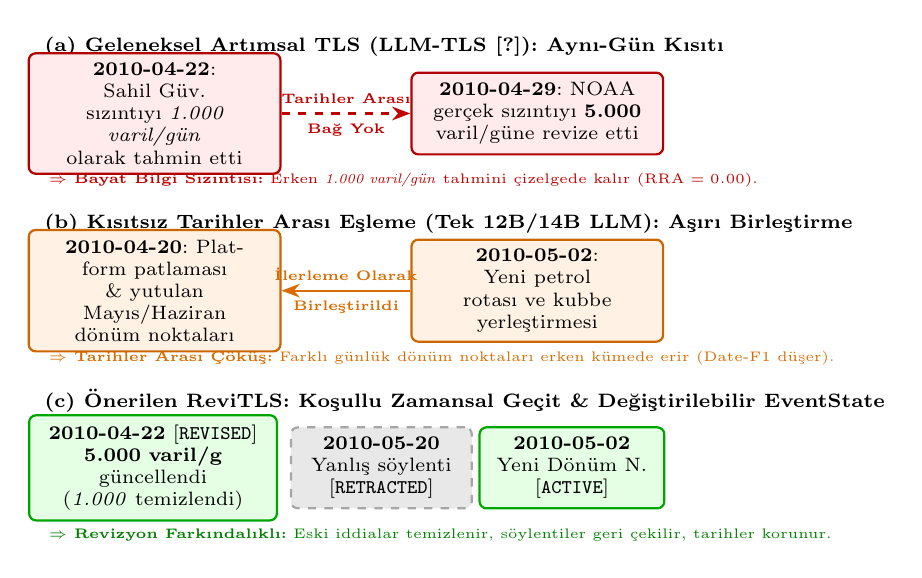
\begin{tikzpicture}[
    font=\scriptsize,
    box/.style={rectangle, rounded corners=2.5pt, draw=black!75, thick, inner sep=3.5pt, align=center},
    failbox/.style={box, fill=red!8, draw=red!70!black},
    warnbox/.style={box, fill=orange!10, draw=orange!80!black},
    okbox/.style={box, fill=green!10, draw=green!65!black},
    arrow/.style={-Stealth, thick}
]
% Panel A
\node[anchor=west, font=\scriptsize\bfseries] at (-0.1, 4.35) {(a) Geleneksel Art{\i}msal TLS (LLM-TLS~\cite{hu2024moments}): Ayn{\i}-G\"{u}n K{\i}s{\i}t{\i}};
\node[failbox, text width=2.95cm] (a1) at (1.42, 3.50) {\textbf{2010-04-22}: Sahil G\"{u}v.\\s{\i}z{\i}nt{\i}y{\i} \textit{1.000 varil/g\"{u}n}\\olarak tahmin etti};
\node[failbox, text width=2.95cm] (a2) at (6.28, 3.50) {\textbf{2010-04-29}: NOAA\\ger\c{c}ek s{\i}z{\i}nt{\i}y{\i} \textbf{5.000}\\varil/g\"{u}ne revize etti};
\draw[arrow, dashed, red!75!black] (a1) -- node[above, font=\tiny\bfseries] {Tarihler Aras{\i}} node[below, font=\tiny\bfseries] {Ba\u{g} Yok} (a2);
\node[anchor=west, font=\tiny, text=red!75!black] at (-0.05, 2.65) {$\Rightarrow$ \textbf{Bayat Bilgi S{\i}z{\i}nt{\i}s{\i}:} Erken \textit{1.000 varil/g\"{u}n} tahmini \c{c}izelgede kal{\i}r ($\text{RRA}=0.00$).};

% Panel B
\node[anchor=west, font=\scriptsize\bfseries] at (-0.1, 2.10) {(b) K{\i}s{\i}ts{\i}z Tarihler Aras{\i} E\c{s}leme (Tek 12B/14B LLM): A\c{s}{\i}r{\i} Birle\c{s}tirme};
\node[warnbox, text width=2.95cm] (b1) at (1.42, 1.25) {\textbf{2010-04-20}: Platform patlamas{\i}\\\& yutulan May{\i}s/Haziran\\d\"{o}n\"{u}m noktalar{\i}};
\node[warnbox, text width=2.95cm] (b2) at (6.28, 1.25) {\textbf{2010-05-02}: Yeni petrol\\rotas{\i} ve kubbe\\yerle\c{s}tirmesi};
\draw[arrow, orange!85!black] (b2) -- node[above, font=\tiny\bfseries] {\.{I}lerleme Olarak} node[below, font=\tiny\bfseries] {Birle\c{s}tirildi} (b1);
\node[anchor=west, font=\tiny, text=orange!85!black] at (-0.05, 0.40) {$\Rightarrow$ \textbf{Tarihler Aras{\i} \c{C}\"{o}k\"{u}\c{s}:} Farkl{\i} g\"{u}nl\"{u}k d\"{o}n\"{u}m noktalar{\i} erken k\"{u}mede erir ($\text{Date-F1}$ d\"{u}\c{s}er).};

% Panel C
\node[anchor=west, font=\scriptsize\bfseries] at (-0.1, -0.15) {(c) \"{O}nerilen ReviTLS: Ko\c{s}ullu Zamansal Ge\c{c}it \& De\u{g}i\c{s}tirilebilir EventState};
\node[okbox, text width=2.90cm] (c1) at (1.40, -1.00) {\textbf{2010-04-22} [\texttt{REVISED}]\\\textbf{5.000 varil/g} g\"{u}ncellendi\\(\textit{1.000} temizlendi)};
\node[box, fill=gray!18, draw=gray!70, dashed, text width=2.05cm] (c2) at (4.30, -1.00) {\textbf{2010-05-20}\\Yanl{\i}\c{s} s\"{o}ylenti\\{[\texttt{RETRACTED}]}};
\node[okbox, text width=2.10cm] (c3) at (6.72, -1.00) {\textbf{2010-05-02}\\Yeni D\"{o}n\"{u}m N.\\{[\texttt{ACTIVE}]}};
\node[anchor=west, font=\tiny, text=green!50!black] at (-0.05, -1.85) {$\Rightarrow$ \textbf{Revizyon Fark{\i}ndal{\i}kl{\i}:} Eski iddialar temizlenir, s\"{o}ylentiler geri \c{c}ekilir, tarihler korunur.};
\end{tikzpicture}%
}
\caption{Geli\c{s}en haber ak{\i}\c{s}lar{\i}nda art{\i}msal zaman \c{c}izelgesi \"{o}zetleme paradigmalar{\i}n{\i}n kar\c{s}{\i}la\c{s}t{\i}r{\i}lmas{\i}. (a) Ayn{\i}-g\"{u}n k\"{u}meleme tarihler aras{\i} d\"{u}zeltmeleri ba\u{g}layamaz ve g\"{u}ncelli\u{g}ini yitirmi\c{s} iddialar{\i} korur. (b) K{\i}s{\i}ts{\i}z tarihler aras{\i} e\c{s}leme farkl{\i} g\"{u}nl\"{u}k geli\c{s}meleri a\c{s}{\i}r{\i} birle\c{s}tirir. (c) \textbf{ReviTLS}, revizyon ipu\c{c}lar{\i} i\c{c}in tarihler aras{\i} eri\c{s}imi se\c{c}ici olarak a\c{c}ar ve de\u{g}i\c{s}tirilebilir olay durumlar{\i}n{\i} g\"{u}nceller.}
\label{fig:paradigm}
\end{figure}

Dura\u{g}an anlat{\i}lardaki etkinliklerine ra\u{g}men, mevcut LLM tabanl{\i} TLS \c{c}erçeveleri kritik bir s{\i}n{\i}rl{\i}l{\i}\u{g}{\i} payla\c{s}maktad{\i}r: haber ak{\i}\c{s}{\i}ndaki olgular{\i}n \c{c}eli\c{s}ki olmaks{\i}z{\i}n monotonik olarak birikti\u{g}ini varsayarlar. Ger\c{c}ek\c{c}i akan veri senaryolar{\i}nda---\"{o}rne\u{g}in end\"{u}striyel felaketler (2010 Deepwater Horizon petrol s{\i}z{\i}nt{\i}s{\i} gibi), halk sa\u{g}l{\i}\u{g}{\i} acil durumlar{\i} veya finansal krizler---gazetecilik habercili\u{g}i do\u{g}as{\i} gere\u{g}i monotonik de\u{g}ildir ve kendini d\"{u}zeltir:
\begin{enumerate}
    \item \textbf{Nicel Revizyonlar:} \"{O}n tahminler (\"{o}rne\u{g}in 22~Nisan'da bildirilen ``g\"{u}nl\"{u}k 1.000 varil'' ilk s{\i}z{\i}nt{\i} oran{\i}) g\"{u}nler sonra resm\^{i} olarak revize edilir (29~Nisan'da ``g\"{u}nl\"{u}k 5.000 varil'').
    \item \textbf{Zamansal ve Nedensel D\"{u}zeltmeler:} Sonraki soru\c{s}turmalar bir olay{\i}n ba\c{s}lang{\i}\c{c}ta bildirilenden daha erken bir tarihte ger\c{c}ekle\c{s}ti\u{g}ini ortaya \c{c}{\i}kar{\i}r veya \"{o}n nedensel at{\i}flar{\i} tersine \c{c}evirir.
    \item \textbf{S\"{o}ylenti Geri \c{C}ekmeleri:} \.{I}kincil olaylara ili\c{s}kin son dakika haberleri (\"{o}rne\u{g}in do\u{g}rulanmam{\i}\c{s} ikinci bir boru hatt{\i} s{\i}z{\i}nt{\i}s{\i}) daha sonra inceleme ekipleri taraf{\i}ndan yalanlan{\i}r ve zaman \c{c}izelgesinden \c{c}{\i}kar{\i}lmal{\i}d{\i}r.
\end{enumerate}

\c{S}ekil~\ref{fig:paradigm}(a)'da g\"{o}sterildi\u{g}i \"{u}zere, mevcut sistemler bu t\"{u}r g\"{u}ncellemelerle ba\c{s}a \c{c}{\i}kamaz. LLM-TLS~\cite{hu2024moments} aday e\c{s}le\c{s}tirmeyi ayn{\i} yay{\i}n tarihiyle s{\i}n{\i}rlad{\i}\u{g}{\i} ve \"{o}zet c\"{u}mlelerini TextRank merkeziyetine g\"{o}re se\c{c}ti\u{g}i i\c{c}in, $t + \Delta t$ an{\i}nda yay{\i}nlanan bir d\"{u}zeltme $t$ an{\i}ndaki orijinal k\"{u}meye eri\c{s}emez; dahas{\i}, yo\u{g}un bi\c{c}imde tekrarlanan erken tahminler tekil yetkili d\"{u}zeltmelerden daha y\"{u}ksek puan alarak ciddi \textit{Bayat Bilgi S{\i}z{\i}nt{\i}s{\i}na} yol a\c{c}ar. Benzer \c{s}ekilde CHRONOS~\cite{wu2025unfolding}, tur d\"{u}zeyindeki zaman \c{c}izelgelerini a\c{c}{\i}k bir \c{c}at{\i}\c{s}ma do\u{g}rulamas{\i} olmadan y\"{u}zeysel tekille\c{s}tirme ile birle\c{s}tirir.

Ampirik analizimiz ayr{\i}ca iki kar\c{s}{\i}t k\"{u}meleme ba\u{s}ar{\i}s{\i}zl{\i}k modunu ortaya koymaktad{\i}r. \.{I}lk olarak, ayn{\i}-g\"{u}n k{\i}s{\i}t{\i} ge\c{c}it olmaks{\i}z{\i}n \c{c}ok ayl{\i}k bir geriye d\"{o}n\"{u}k pencereye (\"{o}rn.\ $90$~g\"{u}n) gev\c{s}etildi\u{g}inde, geni\c{s} anlamsal ili\c{s}kilendirme tek-konulu bir ak{\i}\c{s}taki sonraki g\"{u}nl\"{u}k geli\c{s}melerin erken k\"{u}melerin devam{\i} olarak yanl{\i}\c{s} s{\i}n{\i}fland{\i}r{\i}lmas{\i}na ve farkl{\i} d\"{o}n\"{u}m noktas{\i} tarihlerinin mevcut d\"{u}\u{g}\"{u}mlere \c{c}\"{o}kmesine yol a\c{c}ar (\textbf{Tarihler Aras{\i} A\c{s}{\i}r{\i} Birle\c{s}tirme}, \c{S}ekil~\ref{fig:paradigm}(b)). \.{I}kinci olarak, ultra yo\u{g}un ak{\i}\c{s}larda (Crisis gibi) \c{c}ok-iddial{\i} \c{c}{\i}kar{\i}mla birlikte kat{\i} ayn{\i}-g\"{u}n rutin e\c{s}lemesi ($\Delta t_{\text{routine}}=0$) uygulanmas{\i}, ayn{\i}-g\"{u}n geli\c{s}melerini \c{c}ok say{\i}da d\"{u}\c{s}\"{u}k destekli d\"{u}\u{g}\"{u}me b\"{o}lerek \textbf{Durum Par\c{c}alanmas{\i}na} neden olur ve Denklem~\eqref{eq:salience_score} frekans sinyallerini zay{\i}flat{\i}r.

Her iki g\"{u}\c{c}l\"{u}\u{g}\"{u} \c{c}\"{o}zmek i\c{c}in, ertelenmi\c{s} Faz-2 uzla\c{s}t{\i}rmal{\i} bir akan-veri al{\i}m{\i} boru hatt{\i} olarak tasarlanan \textbf{ReviTLS}'i \"{o}neriyoruz (\c{S}ekil~\ref{fig:paradigm}(c)). Olay k\"{u}melerini de\u{g}i\c{s}tirilemez c\"{u}mle torbalar{\i} olarak ele almak yerine ReviTLS, makaleleri kronolojik olarak yap{\i}land{\i}r{\i}lm{\i}\c{s} $5\text{W}1\text{H}$ yuvalar{\i}, aktif ve temizlenmi\c{s} iddia k\"{u}meleri ve ayr{\i}k ya\c{s}am d\"{o}ng\"{u}s\"{u} durumlar{\i} (\texttt{ACTIVE}, \texttt{REVISED}, \texttt{RETRACTED}) i\c{c}eren de\u{g}i\c{s}tirilebilir \texttt{EventState} d\"{u}\u{g}\"{u}mlerinden olu\c{s}an dinamik bir depoya al{\i}r. Uzun menzilli revizyonlar{\i} desteklerken tarihler aras{\i} a\c{s}{\i}r{\i} birle\c{s}tirmeyi \"{o}nlemek i\c{c}in ReviTLS, rutin olaylar i\c{c}in ayn{\i}-g\"{u}n e\c{s}lemesini zorunlu k{\i}lan, revizyon ipu\c{c}lu makaleleri ise iste\u{g}e ba\u{g}l{\i} \c{c}apraz-kodlay{\i}c{\i} yeniden s{\i}ralama ve ertelenmi\c{s} $14\text{B}$ do\u{g}rulama ile $90$~g\"{u}nl\"{u}k geriye d\"{o}n\"{u}k pencereye s{\i}ralayan ve makale ba\c{s}{\i}na model de\u{g}i\c{s}iminden ka\c{c}{\i}nan bir \textit{Ko\c{s}ullu \c{C}ift-Ufuklu Zamansal Ge\c{c}it} sunar.

\c{C}al{\i}\c{s}mam{\i}z \"{u}\c{c} ara\c{s}t{\i}rma sorusunu incelemektedir: \textbf{AS1:} Ko\c{s}ullu zamansal ge\c{c}it, standart TLS kalitesini korurken tarihler aras{\i} olgusal revizyonlar{\i} ve s\"{o}ylenti geri \c{c}ekmelerini \c{c}\"{o}zebilir mi? \textbf{AS2:} Model \"{o}l\c{c}e\u{g}i, se\c{c}im kurallar{\i} ve ge\c{c}it mekanizmas{\i} durum par\c{c}alanmas{\i}n{\i} ve tarihler aras{\i} a\c{s}{\i}r{\i} birle\c{s}tirmeyi nas{\i}l etkiler? \textbf{AS3:} Revizyon \c{c}\"{o}z\"{u}m\"{u}, parametrik \"{o}n-e\u{g}itim ezberinden ziyade ak{\i}\c{s} i\c{c}i kan{\i}tlar{\i} m{\i} yans{\i}t{\i}r?

Temel katk{\i}lar{\i}m{\i}z \c{s}u \c{s}ekilde \"{o}zetlenebilir:
\begin{itemize}
    \item Monotonik olmayan zaman \c{c}izelgesi \"{o}zetlemeyi form\"{u}le ediyor ve olaylar{\i} a\c{c}{\i}k mezar ta\c{s}{\i} temizleme, ko\c{s}ullu zamansal ge\c{c}it ve ertelenmi\c{s} Faz-2 uzla\c{s}t{\i}rmal{\i} akan veri al{\i}m{\i} ile de\u{g}i\c{s}tirilebilir $5\text{W}1\text{H}$ durum d\"{u}\u{g}\"{u}mleri olarak modelleyen \textbf{ReviTLS}'i \"{o}neriyoruz.
    \item Durum-say{\i}s{\i} tan{\i}lar{\i} arac{\i}l{\i}\u{g}{\i}yla hem \textit{Tarihler Aras{\i} A\c{s}{\i}r{\i} Birle\c{s}tirmeyi} (k{\i}s{\i}ts{\i}z $90$~g\"{u}nl\"{u}k e\c{s}lemede) hem de \textit{Durum Par\c{c}alanmas{\i}n{\i}} (yo\u{g}un Crisis ak{\i}\c{s}lar{\i}nda) ampirik olarak karakterize ediyor; iki fazl{\i} $7\text{B}/14\text{B}$ \c{c}izelgeyi \"{o}l\c{c}ek e\c{s}le\c{s}tirmeli, sonradan-denetimli (post-hoc) ve yaln{\i}zca \"{u}zerine-yazma referanslar{\i}na kar\c{s}{\i} de\u{g}erlendiriyoruz.
    \item $13$ standart TLS konusu ($17{,}679$ makale) \"{u}zerinde tam-derlem de\u{g}erlendirmesi sunuyor; bunun yan{\i}nda kontroll\"{u} sentetik setler ($16$ \c{c}ok-konulu, $8$ kar\c{s}{\i}t-olgusal ve $8$ \"{o}rt\"{u}k-ipu\c{c}lu uzun-gecikmeli senaryo) \"{u}zerinde revizyon do\u{g}rulu\u{g}u, bile\c{s}en ablasyonlar{\i} ve ger\c{c}ek ak{\i}\c{s} hata analizleri sa\u{g}l{\i}yoruz.
\end{itemize}

\section{\.{I}lgili \c{C}al{\i}\c{s}malar}
\label{sec:related}

\subsection{Klasik ve Graf Tabanl{\i} Zaman \c{C}izelgesi \"{O}zetleme}
Erken d\"{o}nem ara\c{s}t{\i}rmalar{\i} dura\u{g}an belge koleksiyonlar{\i} \"{u}zerinde zaman \c{c}izelgesi \"{o}zetlemeyi (TLS) \"{u}\c{c} ana paradigma ile ele alm{\i}\c{s}t{\i}r~\cite{tran2013leveraging, tran2015timeline, martschat2017improving, ghalandari2020examining}: belirginlik ve zamansal \c{c}e\c{s}itlili\u{g}i dengeleyen \c{c}{\i}kar{\i}msal optimizasyon~\cite{martschat2018temporally}, tarih ba\c{s}{\i}na c\"{u}mle s{\i}k{\i}\c{s}t{\i}rma ile birle\c{s}tirilen g\"{o}zetimli tarih se\c{c}imi (\texttt{Datewise})~\cite{ghalandari2020examining, steen2019abstractive} ve olay k\"{u}meleme veya graf s{\i}k{\i}\c{s}t{\i}rma (\texttt{CLUST}, \texttt{MTLS}, \texttt{EGC})~\cite{ghalandari2020examining, yu2021multi, li2021timeline}. Dura\u{g}an k{\i}yaslamalarda etkili olsalar da, bu \c{c}evrimd{\i}\c{s}{\i} y\"{o}ntemler t\"{u}m belge koleksiyonuna ba\c{s}tan eri\c{s}im gerektirir ve art{\i}msal durum revizyonunu desteklemez.

\begin{figure*}[t]
\centering
\resizebox{\textwidth}{!}{%
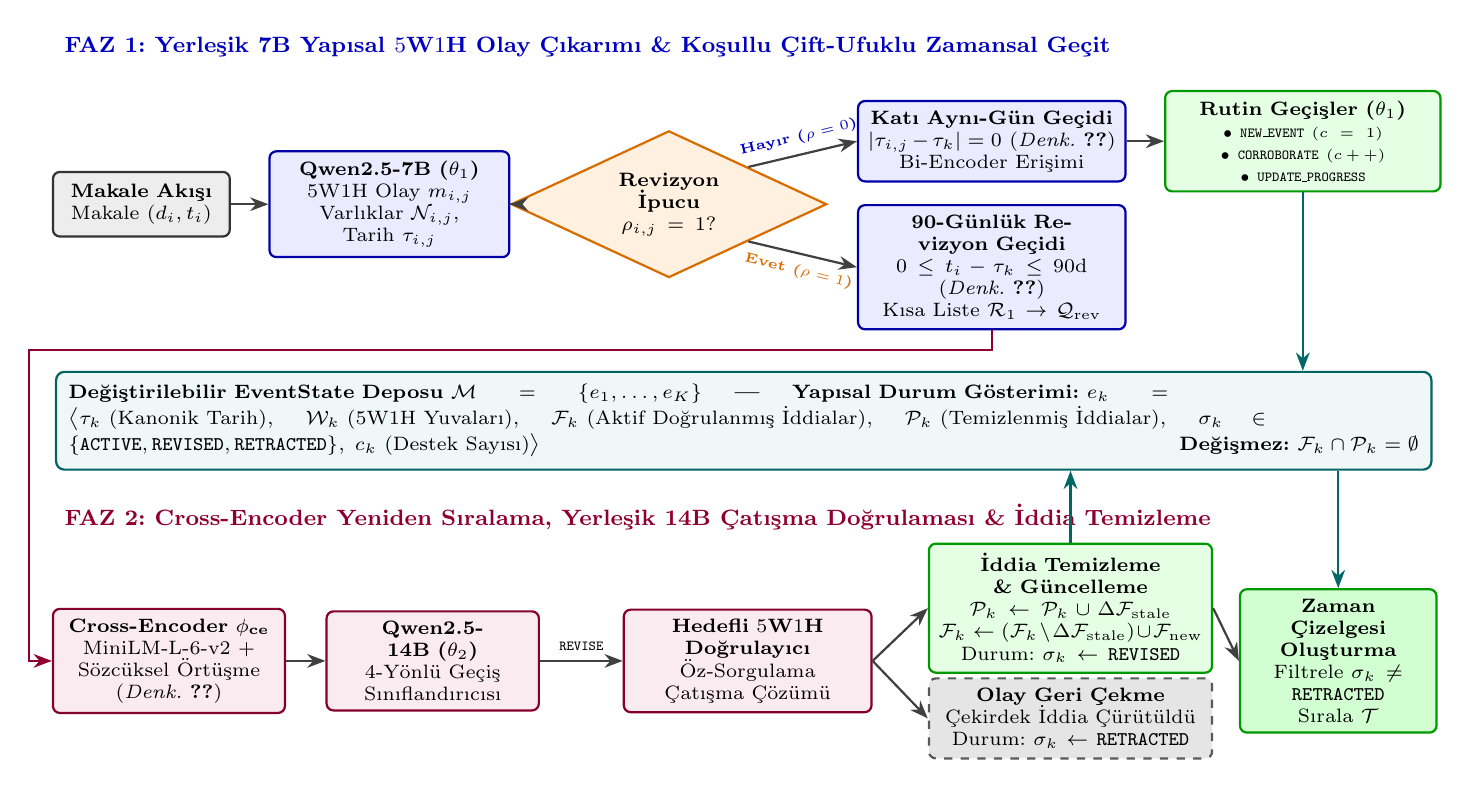
\begin{tikzpicture}[
    font=\scriptsize,
    block/.style={rectangle, rounded corners=2.5pt, draw=black!80, thick, minimum height=0.82cm, align=center, inner sep=3.5pt},
    phase1/.style={block, fill=blue!8, draw=blue!65!black},
    gate/.style={diamond, aspect=2.15, draw=orange!85!black, thick, fill=orange!12, align=center, inner sep=1.5pt},
    phase2/.style={block, fill=purple!8, draw=purple!70!black},
    state/.style={block, fill=green!10, draw=green!60!black},
    membox/.style={rectangle, rounded corners=3pt, draw=teal!80!black, thick, fill=teal!6, align=left, inner sep=4.5pt},
    retract/.style={block, fill=gray!20, draw=gray!70!black, dashed},
    arrow/.style={-Stealth, thick, draw=black!75}
]

% ================= PHASE 1 =================
\node[anchor=west, font=\footnotesize\bfseries, text=blue!75!black] at (-0.15, 6.45) {FAZ 1: Yerle\c{s}ik 7B Yap{\i}sal $5\text{W}1\text{H}$ Olay \c{C}{\i}kar{\i}m{\i} \& Ko\c{s}ullu \c{C}ift-Ufuklu Zamansal Ge\c{c}it};

\node[block, fill=gray!14, text width=2.0cm] (stream) at (0.95, 4.45) {\textbf{Makale Ak{\i}\c{s}{\i}}\\Makale $(d_i, t_i)$};
\node[phase1, text width=2.8cm] (extractor) at (4.10, 4.45) {\textbf{Qwen2.5-7B ($\theta_1$)}\\$5\text{W}1\text{H}$ Olay $m_{i,j}$\\Varl{\i}klar $\mathcal{N}_{i,j}$, Tarih $\tau_{i,j}$};
\node[gate, text width=1.95cm] (revgate) at (7.65, 4.45) {\textbf{Revizyon \.{I}pucu}\\$\rho_{i,j} = 1$?};

\node[phase1, text width=3.15cm] (sameday) at (11.75, 5.25) {\textbf{Kat{\i} Ayn{\i}-G\"{u}n Ge\c{c}idi}\\$|\tau_{i,j} - \tau_k| = 0$ (\textit{Denk.~\ref{eq:temporal_gate}})\\Bi-Encoder Eri\c{s}imi};
\node[phase1, text width=3.15cm] (deferq) at (11.75, 3.65) {\textbf{90-G\"{u}nl\"{u}k Revizyon Ge\c{c}idi}\\$0 \le t_i - \tau_k \le 90\text{d}$ (\textit{Denk.~\ref{eq:temporal_gate}})\\K{\i}sa Liste $\mathcal{R}_1 \rightarrow \mathcal{Q}_{\text{rev}}$};

\node[state, text width=3.25cm] (sameday_act) at (15.70, 5.25) {\textbf{Rutin Ge\c{c}i\c{s}ler ($\theta_1$)}\\{\tiny $\bullet$ \texttt{NEW\_EVENT} ($c=1$)}\\{\tiny $\bullet$ \texttt{CORROBORATE} ($c\!+\!+$)}\\{\tiny $\bullet$ \texttt{UPDATE\_PROGRESS}}};

\draw[arrow] (stream) -- (extractor);
\draw[arrow] (extractor) -- (revgate);
\draw[arrow] (revgate.north east) -- node[above, sloped, font=\tiny\bfseries, text=blue!75!black] {Hay{\i}r ($\rho=0$)} (sameday.west);
\draw[arrow] (revgate.south east) -- node[below, sloped, font=\tiny\bfseries, text=orange!85!black] {Evet ($\rho=1$)} (deferq.west);
\draw[arrow] (sameday) -- (sameday_act);

% ================= MIDDLE: MUTABLE EVENTSTATE MEMORY =================
\node[membox, text width=17.15cm] (memschema) at (8.60, 1.70) {
    \textbf{De\u{g}i\c{s}tirilebilir EventState Deposu $\mathcal{M} = \{e_1, \dots, e_K\}$ \quad --- \quad Yap{\i}sal Durum G\"{o}sterimi:}
    $e_k = \big\langle \tau_k \text{ (Kanonik Tarih)},\; \mathcal{W}_k \text{ ($5\text{W}1\text{H}$ Yuvalar{\i})},\; \mathcal{F}_k \text{ (Aktif Do\u{g}rulanm{\i}\c{s} \.{I}ddialar)},\; \mathcal{P}_k \text{ (Temizlenmi\c{s} \.{I}ddialar)},\; \sigma_k \in \{\texttt{ACTIVE}, \texttt{REVISED}, \texttt{RETRACTED}\},\; c_k \text{ (Destek Say{\i}s{\i})} \big\rangle$ \hfill \textbf{De\u{g}i\c{s}mez:} $\mathcal{F}_k \cap \mathcal{P}_k = \emptyset$
};

\coordinate (qbus) at ([yshift=0.26cm]memschema.north);
\draw[arrow, teal!80!black] (sameday_act.south) -- (sameday_act.south |- memschema.north);

% ================= PHASE 2 =================
\node[anchor=west, font=\footnotesize\bfseries, text=purple!75!black] at (-0.15, 0.48) {FAZ 2: Cross-Encoder Yeniden S{\i}ralama, Yerle\c{s}ik 14B \c{C}at{\i}\c{s}ma Do\u{g}rulamas{\i} \& \.{I}ddia Temizleme};

\node[phase2, text width=2.70cm] (crossenc) at (1.30, -1.35) {\textbf{Cross-Encoder $\phi_{\text{ce}}$}\\MiniLM-L-6-v2 +\\S\"{o}zc\"{u}ksel \"{O}rt\"{u}\c{s}me (\textit{Denk.~\ref{eq:hybrid_rerank}})};
\node[phase2, text width=2.45cm] (cls14b) at (4.65, -1.35) {\textbf{Qwen2.5-14B ($\theta_2$)}\\4-Y\"{o}nl\"{u} Ge\c{c}i\c{s}\\S{\i}n{\i}fland{\i}r{\i}c{\i}s{\i}};
\node[phase2, text width=2.90cm] (verifier) at (8.65, -1.35) {\textbf{Hedefli $5\text{W}1\text{H}$ Do\u{g}rulay{\i}c{\i}}\\\"{O}z-Sorgulama\\ \c{C}at{\i}\c{s}ma \c{C}\"{o}z\"{u}m\"{u}};

\node[state, text width=3.35cm] (purge) at (12.75, -0.68) {\textbf{\.{I}ddia Temizleme \& G\"{u}ncelleme}\\$\mathcal{P}_k \leftarrow \mathcal{P}_k \cup \Delta\mathcal{F}_{\text{stale}}$\\$\mathcal{F}_k \leftarrow (\mathcal{F}_k \setminus \Delta\mathcal{F}_{\text{stale}}) \cup \mathcal{F}_{\text{new}}$\\Durum: $\sigma_k \leftarrow \texttt{REVISED}$};
\node[retract, text width=3.35cm] (retracted) at (12.75, -2.08) {\textbf{Olay Geri \c{C}ekme}\\\c{C}ekirdek \.{I}ddia \c{C}\"{u}r\"{u}t\"{u}ld\"{u}\\Durum: $\sigma_k \leftarrow \texttt{RETRACTED}$};

\node[state, fill=green!18, text width=2.25cm] (ranker) at (16.15, -1.35) {\textbf{Zaman \c{C}izelgesi}\\\textbf{Olu\c{s}turma}\\Filtrele $\sigma_k \neq \texttt{RETRACTED}$\\S{\i}rala $\mathcal{T}$};

\draw[arrow, purple!75!black] (deferq.south) -- (deferq.south |- qbus) -- (-0.48, 0 |- qbus) -- (-0.48, -1.35) -- (crossenc.west);
\draw[arrow] (crossenc) -- (cls14b);
\draw[arrow] (cls14b) -- node[above, font=\tiny\bfseries] {\texttt{REVISE}} (verifier);
\draw[arrow] (verifier.east) -- (purge.west);
\draw[arrow] (verifier.east) -- (retracted.west);
\draw[arrow, teal!80!black] (purge.north) -- (purge.north |- memschema.south);
\draw[arrow, teal!80!black] (ranker.north |- memschema.south) -- (ranker.north);
\draw[arrow] (purge.east) -- (ranker.west);

\end{tikzpicture}%
}
\caption{\textbf{ReviTLS} boru hatt{\i}na genel bak{\i}\c{s}. Faz~1'de gelen makaleler $7\text{B}$ model taraf{\i}ndan yap{\i}land{\i}r{\i}lm{\i}\c{s} $5\text{W}1\text{H}$ olay adaylar{\i}na \"{o}zetlenir ve Ko\c{s}ullu \c{C}ift-Ufuklu Zamansal Ge\c{c}it ($\Delta t_{\text{routine}}=0\text{g}$ vs.\ $\Delta t_{\text{rev}}=90\text{g}$) ile y\"{o}nlendirilir. Rutin ayn{\i}-g\"{u}n g\"{u}ncellemeleri do\u{g}rudan de\u{g}i\c{s}tirilebilir \texttt{EventState} deposuna i\c{s}lenirken, tarihler aras{\i} revizyon adaylar{\i} Faz~2 \c{c}apraz-kodlay{\i}c{\i} yeniden s{\i}ralama ve $14\text{B}$ \c{c}at{\i}\c{s}ma do\u{g}rulamas{\i} i\c{c}in kuyru\u{g}a al{\i}n{\i}r.}
\label{fig:architecture}
\end{figure*}

\subsection{LLM Tabanl{\i} Art{\i}msal ve Eri\c{s}im-Destekli TLS}
Son \c{c}al{\i}\c{s}malar art{\i}msal ve a\c{c}{\i}k-alan zaman \c{c}izelgesi \"{u}retimi i\c{c}in talimat-ayarl{\i} LLM'lerden yararlanm{\i}\c{s}t{\i}r. Hu vd.~\cite{hu2024moments}, d\"{o}n\"{u}m noktas{\i} \"{o}zetlerini TextRank ile se\c{c}meden \"{o}nce gelen haber makalelerini ayn{\i}-tarih sezgisi alt{\i}nda art{\i}msal olarak k\"{u}meleyen \textbf{LLM-TLS}'i tan{\i}tm{\i}\c{s}t{\i}r. Eri\c{s}im-destekli paradigmada Wu vd.~\cite{wu2025unfolding}, bir belge koleksiyonu \"{u}zerinden yinelemeli olarak $5\text{W}1\text{H}$ \"{o}z-sorular{\i} \"{u}reten ve tur d\"{u}zeyindeki zaman \c{c}izelgelerini birle\c{s}tiren \textbf{CHRONOS}'u \"{o}nermi\c{s}tir. Ortogonal uzant{\i}lar aras{\i}nda zaman \c{c}izelgesi ayr{\i}nt{\i} d\"{u}zeyini kullan{\i}c{\i}n{\i}n belirtti\u{g}i s{\i}k{\i}\c{s}t{\i}rma seviyelerine uyarlayan \textbf{DTELS}~\cite{dtels2025} ve bo\c{s}luk doldurma i\c{c}in k\"{u}resel olay belle\u{g}ine sahip ak{\i}l y\"{u}r\"{u}tme modellerinden yararlanan \textbf{TimelineReasoner}~\cite{zhang2026timelinereasoner} yer almaktad{\i}r. Bu \c{c}erçeveler art{\i}msal k\"{u}meleme, ayr{\i}nt{\i} kontrol\"{u} ve yinelemeli eri\c{s}imi ilerletse de, hi\c{c}biri monotonik olmayan tarihler aras{\i} d\"{u}zeltmeler i\c{c}in mezar ta\c{s}{\i} tabanl{\i} iddia temizleme veya ya\c{s}am d\"{o}ng\"{u}s\"{u} geri \c{c}ekmesini a\c{c}{\i}k\c{c}a i\c{c}ermemektedir.

\subsection{G\"{u}ncelleme \"{O}zetleme, \.{I}nan\c{c} Revizyonu ve Bilgi \c{C}at{\i}\c{s}malar{\i}}
Monotonik olmayan bilgi evrimi bir\c{c}ok ilgili gelenekte incelenmi\c{s}tir. Erken d\"{o}nem Konu Tespiti ve Takibi (TDT)~\cite{allan2002topic}, TAC G\"{u}ncelleme \"{O}zetleme~\cite{dang2008overview} ve TREC Zamansal \"{O}zetleme~\cite{aslam2013trec, kedzie2015predicting}, tarihsel d\"{o}n\"{u}m noktalar{\i}ndaki ge\c{c}ersiz iddialar{\i} geri \c{c}ekmekten ziyade felaket ak{\i}\c{s}lar{\i}nda tekrar{\i} \"{o}nleyerek yeni g\"{u}ncellemeler yay{\i}nlamaya odaklanm{\i}\c{s}t{\i}r. Mezar ta\c{s}{\i} mekanizmam{\i}za kavramsal olarak en yak{\i}n yakla\c{s}{\i}mlar, \c{c}eli\c{s}en kan{\i}t geldi\u{g}inde ge\c{c}ersiz gerek\c{c}eleri a\c{c}{\i}k\c{c}a izleyen ve geri \c{c}eken klasik Do\u{g}ruluk Bak{\i}m Sistemleri (TMS)~\cite{doyle1979truth} ve AGM inan\c{c} revizyonudur~\cite{alchourron1985logic}. Modern NLP'de s\"{o}ylenti do\u{g}rulama~\cite{zubiaga2016analysing, kochkina2018all, thorne2018fever}, do\u{g}ruluk ke\c{s}fi~\cite{li2016survey}, zamansal bilgi taban{\i} g\"{u}ncelleme~\cite{dhingra2022time, kasai2023realtime}, ba\u{g}lamsal bilgi-\c{c}at{\i}\c{s}mas{\i} \c{c}\"{o}z\"{u}m\"{u}~\cite{xu2024knowledge} ve parametrik model d\"{u}zenleme~\cite{meng2022locating, mitchell2022fast} \c{c}eli\c{s}en iddialar{\i} iddia veya a\u{g}{\i}rl{\i}k d\"{u}zeyinde ele al{\i}r. ReviTLS, Tablo~\ref{tab:related_work}'de kar\c{s}{\i}la\c{s}t{\i}r{\i}ld{\i}\u{g}{\i} \"{u}zere a\c{c}{\i}k durum geri \c{c}ekme ve \c{c}at{\i}\c{s}ma do\u{g}rulamas{\i}n{\i} akan zaman \c{c}izelgesi \"{o}zetlemeye ta\c{s}{\i}r.

\begin{table}[t]
\centering
\caption{ReviTLS'in Temsilci TLS Paradigmalar{\i}yla Kar\c{s}{\i}la\c{s}t{\i}r{\i}lmas{\i}}
\label{tab:related_work}
\renewcommand{\arraystretch}{1.10}
\resizebox{\columnwidth}{!}{%
\begin{tabular}{@{}lccccc@{}}
\toprule
\textbf{Y\"{o}ntem} & \textbf{Tarihler Aras{\i}} & \textbf{\.{I}ddia Geri} & \textbf{De\u{g}i\c{s}tirilebilir} & \textbf{Akan Veri} & \textbf{Revizyon} \\
 & \textbf{Ba\u{g}lama} & \textbf{\c{C}ekme} & \textbf{Ge\c{c}mi\c{s}} & \textbf{Al{\i}m{\i}} & \textbf{De\u{g}.} \\
\midrule
\textbf{DATEWISE / EGC}~\cite{ghalandari2020examining, li2021timeline} & $\times$ & $\times$ & $\times$ & $\times$ & $\times$ \\
\textbf{CHRONOS}~\cite{wu2025unfolding} & \checkmark & $\times$ & $\times$ & $\times$ & $\times$ \\
\textbf{DTELS / TR}~\cite{dtels2025, zhang2026timelinereasoner} & \checkmark & $\times$ & $\times$ & $\times$ & $\times$ \\
\textbf{LLM-TLS}~\cite{hu2024moments} & $\times$ & $\times$ & $\times$ & \checkmark & $\times$ \\
\textbf{ReviTLS (Bizim)} & \checkmark & \checkmark & \checkmark & \checkmark$^*$ & \checkmark \\
\bottomrule
\multicolumn{6}{@{}l}{\scriptsize $^*$Akan Faz-1 veri al{\i}m{\i} ile ertelenmi\c{s} (veya iste\u{g}e ba\u{g}l{\i} \c{c}evrimi\c{c}i) Faz-2 uzla\c{s}t{\i}rma.}
\end{tabular}%
}
\end{table}

\section{Problem Tan{\i}m{\i}}
\label{sec:problem}

Konu zaman \c{c}izelgesi \"{o}zetleme alan{\i}ndaki \"{o}nceki \c{c}al{\i}\c{s}malar{\i}~\cite{ghalandari2020examining, hu2024moments} izleyerek, girdi hedef bir konuya ili\c{s}kin kronolojik olarak s{\i}ralanm{\i}\c{s} bir haber makalesi ak{\i}\c{s}{\i} $\mathcal{S} = \{(d_1, t_1), (d_2, t_2), \dots, (d_N, t_N)\}$ (burada $d_i$ makale metni, $t_i$ yay{\i}n tarihidir; $t_1 \le t_2 \le \dots \le t_N$) ve d\"{o}n\"{u}m noktas{\i} tarihlerinin say{\i}s{\i}n{\i} belirten hedef zaman \c{c}izelgesi uzunlu\u{g}u $l$'dir. Akan yan{\i}t h{\i}z{\i}n{\i} GPU bellek verimlili\u{g}iyle dengelemek i\c{c}in Faz~1 gelen makaleleri yaln{\i}zca kronolojik \"{o}n-ekler $\mathcal{S}_{\le i}$ \"{u}zerinden i\c{s}lerken, Faz~2 ak{\i}\c{s} sonunda son zaman \c{c}izelgesi olu\c{s}turulmadan \"{o}nce s{\i}ralanan revizyon adaylar{\i} $\mathcal{Q}_{\text{rev}}$ \"{u}zerinde ertelenmi\c{s} toplu do\u{g}rulama ger\c{c}ekle\c{s}tirir.

Olaylar{\i} bir kez \c{c}{\i}kar{\i}ld{\i}ktan sonra de\u{g}i\c{s}mez kabul eden geleneksel art{\i}msal TLS'nin aksine, $t_i$ tarihinde yay{\i}nlanan bir $d_i$ makalesi ya $t_i$ g\"{u}n\"{u}nde ger\c{c}ekle\c{s}en yeni bir geli\c{s}meyi bildirebilir ya da $\tau_k \le t_i$ tarihindeki tarihsel bir olaya ili\c{s}kin geriye d\"{o}n\"{u}k bir d\"{u}zeltme, nicel g\"{u}ncelleme veya geri \c{c}ekme sa\u{g}layabilir. Monotonik olmayan g\"{u}ncellemeleri desteklemek i\c{c}in her olay k\"{u}mesini $e_k \in \mathcal{M}$ de\u{g}i\c{s}tirilebilir bir \textbf{\texttt{EventState}} demeti olarak temsil ediyoruz:
\begin{equation}
e_k = \langle \tau_k,\; \mathcal{W}_k,\; \mathcal{F}_k,\; \mathcal{P}_k,\; \sigma_k,\; c_k \rangle,
\label{eq:event_state}
\end{equation}
burada $\tau_k$ kanonik olay tarihidir; $\mathcal{W}_k = \{w_{\text{who}}, w_{\text{what}}, w_{\text{when}}, w_{\text{where}}, w_{\text{why}}, w_{\text{how}}\}$ sentezlenen $5\text{W}1\text{H}$ olay arg\"{u}manlar{\i}n{\i} saklar; $\mathcal{F}_k$ aktif do\u{g}rulanm{\i}\c{s} iddialar k\"{u}mesidir; $\mathcal{P}_k$ ise $\mathcal{F}_k$'den temizlenen g\"{u}ncelli\u{g}ini yitirmi\c{s} iddialar{\i}n mezar ta\c{s}{\i} k\"{u}mesidir ($\mathcal{F}_k \cap \mathcal{P}_k = \emptyset$); $\sigma_k \in \{\texttt{ACTIVE}, \texttt{REVISED}, \texttt{RETRACTED}\}$ ya\c{s}am d\"{o}ng\"{u}s\"{u} durumudur; $c_k$ ise k\"{u}m\"{u}latif destek say{\i}s{\i}d{\i}r. Ama\c{c}, geri \c{c}ekilmemi\c{s} durumlardan ($\sigma_k \neq \texttt{RETRACTED}$) olu\c{s}an, zamansal hizalamay{\i} ve olgusal kapsam{\i} enb\"{u}y\"{u}klerken $\bigcup_k \mathcal{P}_k$'den bayat bilgi s{\i}z{\i}nt{\i}s{\i}n{\i} enk\"{u}\c{c}\"{u}kleyen bir zaman \c{c}izelgesi $\mathcal{T} = \{(\tau_{(1)}, s_{(1)}), \dots, (\tau_{(l)}, s_{(l)})\}$ olu\c{s}turmakt{\i}r.

\section{Y\"{o}ntem}
\label{sec:methodology}

\c{S}ekil~\ref{fig:architecture}'te g\"{o}sterilen ve Algoritma~\ref{alg:revitls}'de bi\c{c}imselle\c{s}tirilen iki fazl{\i}, \c{c}ift-\"{o}l\c{c}ekli \textbf{ReviTLS} zaman \c{c}izelgesi \"{o}zetleme boru hatt{\i}n{\i} \"{o}neriyoruz. Y\"{o}ntemimiz d\"{o}rt temel bile\c{s}enden olu\c{s}ur: (1) yap{\i}land{\i}r{\i}lm{\i}\c{s} $5\text{W}1\text{H}$ olay \c{c}{\i}kar{\i}m{\i}, (2) ko\c{s}ullu \c{c}ift-ufuklu zamansal ge\c{c}it ve iki a\c{s}amal{\i} eri\c{s}im, (3) ertelenmi\c{s} \c{c}at{\i}\c{s}ma do\u{g}rulamas{\i} ve durum ge\c{c}i\c{s}i, ve (4) tarih-tekille\c{s}tirmeli zaman \c{c}izelgesi olu\c{s}turma.

\subsection{Yap{\i}land{\i}r{\i}lm{\i}\c{s} $5\text{W}1\text{H}$ Olay \c{C}{\i}kar{\i}m{\i}}
\label{subsec:extraction}

Yeni bir makale $(d_i, t_i)$ geldi\u{g}inde, Algoritma~\ref{alg:revitls}'de \textsc{Extract5W1H} olarak g\"{o}sterilen talimat-ayarl{\i} bir LLM $\theta_1$ (\texttt{Qwen2.5-7B-Instruct}~\cite{qwen25}) kullanarak yap{\i}land{\i}r{\i}lm{\i}\c{s} atomik olay adaylar{\i} $\mathcal{C}_i = \{m_{i,j}\}$ \c{c}{\i}kar{\i}r{\i}z. Arka plan ba\u{g}lam{\i}n{\i} yeni geli\c{s}melerle kar{\i}\c{s}t{\i}rabilecek serbest bi\c{c}imli c\"{u}mleler \c{c}{\i}karmak yerine $\theta_1$, a\c{c}{\i}k $5\text{W}1\text{H}$ yuvalar{\i}n{\i} $\tilde{\mathcal{W}}_{i,j}$, kanonik varl{\i}klar{\i} ve say{\i}sal de\u{g}erleri $\mathcal{N}_{i,j}$, atomik olgusal iddialar{\i} $\tilde{\mathcal{F}}_{i,j}$ ve \c{c}\"{o}z\"{u}mlenen olay tarihini $\tau_{i,j} \le t_i$ doldurmak i\c{c}in bir JSON \c{s}emas{\i}yla k{\i}s{\i}tlan{\i}r.

Gelen bir $m_{i,j}$ aday{\i}n{\i}n daha \"{o}nce kaydedilmi\c{s} bir olay{\i} potansiyel olarak revize edip etmedi\u{g}ini veya geri \c{c}ekip \c{c}ekmedi\u{g}ini belirlemek i\c{c}in, LLM'in yap{\i}sal bayra\u{g}{\i}n{\i} d\"{u}zeltici i\c{s}aretleyicilerden olu\c{s}an bir s\"{o}zl\"{u}kle $\mathcal{V}_{\text{rev}}$ (\"{o}rn.\ \textit{revise, upward, downward, correct, retract, debunk, false alarm, rule out, previously estimated}) birle\c{s}tiren ikili bir revizyon ipucu g\"{o}stergesi $\rho_{i,j} \in \{0, 1\}$ hesaplar{\i}z:
\begin{equation}
\rho_{i,j} = \mathbb{I}\Big( \hat{\rho}_{\theta_1}(m_{i,j}) = 1 \;\lor\; \big|\text{Tokens}(m_{i,j}) \cap \mathcal{V}_{\text{rev}}\big| > 0 \Big).
\label{eq:rev_cue}
\end{equation}

\subsection{Ko\c{s}ullu Zamansal Ge\c{c}it ve \.{I}ki A\c{s}amal{\i} Eri\c{s}im}
\label{subsec:retrieval}

\c{C}al{\i}\c{s}mam{\i}z{\i}n temel bir bulgusu, t\"{u}m adaylara tekd\"{u}ze $90$~g\"{u}nl\"{u}k geriye d\"{o}n\"{u}k pencere uygulaman{\i}n daha b\"{u}y\"{u}k LLM'lerin geli\c{s}en bir konunun farkl{\i} g\"{u}nl\"{u}k d\"{o}n\"{u}m noktalar{\i}n{\i} erken olay k\"{u}melerinde birle\c{s}tirmesine (\textit{Tarihler Aras{\i} A\c{s}{\i}r{\i} Birle\c{s}tirme}) yol a\c{c}mas{\i}, LLM-TLS'deki~\cite{hu2024moments} gibi eri\c{s}imi $\tau_k = \tau_{i,j}$ ile s{\i}n{\i}rlaman{\i}n ise tarihler aras{\i} revizyonlar{\i} engellemesidir. Bu dengeyi bir \textbf{Ko\c{s}ullu \c{C}ift-Ufuklu Zamansal Ge\c{c}it} $\mathcal{G}(m_{i,j}, e_k) \in \{0, 1\}$ ile \c{c}\"{o}z\"{u}yoruz:
\begin{equation}
\mathcal{G}(m_{i,j}, e_k) = \begin{cases}
\mathbb{I}\big( |\tau_{i,j} - \tau_k| \le \Delta t_{\text{routine}} \big), & \text{e\u{g}er } \rho_{i,j} = 0, \\[3pt]
\mathbb{I}\big( 0 \le t_i - \tau_k \le \Delta t_{\text{rev}} \big), & \text{e\u{g}er } \rho_{i,j} = 1,
\end{cases}
\label{eq:temporal_gate}
\end{equation}
burada $\Delta t_{\text{routine}} = 0$~g\"{u}n rutin geli\c{s}meler ($\rho_{i,j} = 0$) i\c{c}in kat{\i} ayn{\i}-g\"{u}n yerelle\c{s}tirmesi zorunlu k{\i}lar, $\Delta t_{\text{rev}} = 90$~g\"{u}n ise yaln{\i}zca revizyon ipucu ta\c{s}{\i}yan adaylar ($\rho_{i,j} = 1$) i\c{c}in \"{u}\c{c} ayl{\i}k bir geriye d\"{o}n\"{u}k pencere a\c{c}ar.

\begin{algorithm}[t]
\footnotesize
\caption{\textbf{ReviTLS} \.{I}ki Fazl{\i} Boru Hatt{\i}}
\label{alg:revitls}
\DontPrintSemicolon
\KwIn{Makale ak{\i}\c{s}{\i} $\mathcal{S} = \{(d_i, t_i)\}_{i=1}^N$, modeller $\theta_1$ ($7\text{B}$), $\theta_2$ ($14\text{B}$), kodlay{\i}c{\i}lar $\phi_{\text{bi}}, \phi_{\text{ce}}$, uzunluk $l$.}
\KwOut{$l$ tarih damgal{\i} \"{o}zet i\c{c}eren zaman \c{c}izelgesi $\mathcal{T}$.}
$\mathcal{M} \leftarrow \emptyset$, $\mathcal{Q}_{\text{rev}} \leftarrow \emptyset$\;
\tcp{Faz 1: 7B \c{C}{\i}kar{\i}m \& Ayn{\i}-G\"{u}n K\"{u}meleme}
\For{$i = 1$ \KwTo $N$}{
    $\mathcal{C}_i \leftarrow \textsc{Extract5W1H}(d_i, t_i, \theta_1)$\;
    \ForEach{$m_{i,j} \in \mathcal{C}_i$}{
        $\rho_{i,j} \leftarrow \textsc{DetectRevisionCue}(m_{i,j})$ \tcp*{Denk.~\ref{eq:rev_cue}}
        $\mathcal{R}_1 \leftarrow \textsc{RetrieveBiEncoder}(m_{i,j}, \mathcal{M}, \rho_{i,j}, \phi_{\text{bi}})$\;
        \eIf{$\rho_{i,j} == 1$ \textbf{ve} $\mathcal{R}_1 \neq \emptyset$}{
            $\mathcal{Q}_{\text{rev}} \leftarrow \mathcal{Q}_{\text{rev}} \cup \{(m_{i,j}, \mathcal{R}_1)\}$\;
        }{
            $a, e^* \leftarrow \textsc{ClassifyRoutine}(m_{i,j}, \mathcal{R}_1, \theta_1)$\;
            \eIf{$a == \texttt{REVISE\_CONFLICT}$}{
                $\Delta\mathcal{F}_{\text{stale}}, \mathcal{F}_{\text{new}}, \sigma_k \leftarrow \textsc{Verify5W1H}(m_{i,j}, e^*, \theta_1)$\;
                $\mathcal{M} \leftarrow \textsc{PurgeUpdate}(\mathcal{M}, e^*, \Delta\mathcal{F}_{\text{stale}}, \mathcal{F}_{\text{new}}, \sigma_k)$\;
            }{
                $\mathcal{M} \leftarrow \textsc{UpdateState}(\mathcal{M}, m_{i,j}, e^*, a)$\;
            }
        }
    }
}
\tcp{Faz 2: Cross-Encoder S{\i}ralama \& 14B Do\u{g}rulama}
\ForEach{$(m_{i,j}, \mathcal{R}_1) \in \mathcal{Q}_{\text{rev}}$}{
    $\mathcal{R}_2 \leftarrow \textsc{RerankCrossEncoder}(m_{i,j}, \mathcal{R}_1, \phi_{\text{ce}})$ \tcp*{Denk.~\ref{eq:hybrid_rerank}}
    $\text{matched} \leftarrow \textbf{false}$\;
    \ForEach{$e_k^* \in \mathcal{R}_2$}{
        $a \leftarrow \textsc{ClassifyTransition}(m_{i,j}, e_k^*, \theta_2)$\;
        \If{$a == \texttt{REVISE\_CONFLICT}$ \textbf{veya} ($a \neq \texttt{NEW\_EVENT}$ \textbf{ve} $\tau_k^* == \tau_{i,j}$)}{
            \If{$a == \texttt{REVISE\_CONFLICT}$}{
                $\Delta\mathcal{F}_{\text{stale}}, \mathcal{F}_{\text{new}}, \sigma_k \leftarrow \textsc{Verify5W1H}(m_{i,j}, e_k^*, \theta_2)$\;
                $\mathcal{M} \leftarrow \textsc{PurgeUpdate}(\mathcal{M}, e_k^*, \Delta\mathcal{F}_{\text{stale}}, \mathcal{F}_{\text{new}}, \sigma_k)$\;
            }
            \Else{
                $\mathcal{M} \leftarrow \textsc{UpdateState}(\mathcal{M}, m_{i,j}, e_k^*, a)$\;
            }
            $\text{matched} \leftarrow \textbf{true}$; \textbf{break}\;
        }
    }
    \If{\textbf{de\u{g}il} $\text{matched}$}{
        $\mathcal{M} \leftarrow \textsc{UpdateState}(\mathcal{M}, m_{i,j}, \varnothing, \texttt{NEW\_EVENT})$\;
    }
}
\tcp{Zaman \c{C}izelgesi Olu\c{s}turma}
$\mathcal{M}_{\text{valid}} \leftarrow \{e_k \in \mathcal{M} \mid \sigma_k \neq \texttt{RETRACTED}\}$\;
$\mathcal{C}_{\text{top}} \leftarrow \textsc{RankAndDeduplicateDates}(\mathcal{M}_{\text{valid}}, l)$ \tcp*{Denk.~\ref{eq:salience_score}}
$\mathcal{T} \leftarrow \textsc{SortByTime}(\mathcal{C}_{\text{top}})$\;
\Return{$\mathcal{T}$}\;
\end{algorithm}

Zamansal ge\c{c}itten ge\c{c}en geri \c{c}ekilmemi\c{s} durum havuzu \"{u}zerinde iki a\c{s}amal{\i} eri\c{s}im ve karar filtreleme uyguluyoruz:
\begin{enumerate}
    \item \textbf{A\c{s}ama 1 (Varl{\i}k-Destekli Bi-Encoder):} $m_{i,j}$ ve ge\c{c}itten ge\c{c}en her $e_k$ durumunu \texttt{BAAI/bge-base-en-v1.5}~\cite{xiao2024cpack} ($\phi_{\text{bi}}$) kullanarak L2-normalize vekt\"{o}rlere kodluyor ve payla\c{s}{\i}lan her kanonik varl{\i}k i\c{c}in $\lambda_{\text{ent}} = 0.05$ olmak \"{u}zere $S_{\text{bi}} = \cos(\mathbf{v}_{m}, \mathbf{v}_{e_k}) + \lambda_{\text{ent}}\, |\mathcal{N}_{i,j} \cap \mathcal{N}_k|$ skorunu hesapl{\i}yoruz. Yaln{\i}zca $\gamma_{\text{sim}} = 0.45$ benzerlik taban{\i}n{\i} a\c{s}an adaylar korunarak en fazla $K_1 = 10$ boyutunda $\mathcal{R}_1$ k{\i}sa listesi olu\c{s}turulur. Bu taban, konusal olarak ilgisiz k\"{u}meleri budarken tarihler aras{\i} a\c{c}{\i}klamalar{\i} ve d\"{u}zeltmeleri korur.
    \item \textbf{A\c{s}ama 2 (Cross-Encoder Yeniden S{\i}ralama):} Tek-konulu bir ak{\i}\c{s}taki makaleler y\"{u}ksek arka plan g\"{o}mme benzerli\u{g}i payla\c{s}t{\i}\u{g}{\i}ndan, $|\mathcal{R}_1| > 1$ olan k{\i}sa listeler bir \c{c}apraz-dikkat yeniden s{\i}ralay{\i}c{\i}s{\i} $\phi_{\text{ce}}$ (\texttt{ms-marco-MiniLM-L-6-v2}~\cite{wang2020minilm, nguyen2016msmarco}) ve i\c{c}erik-kelimesi s\"{o}zc\"{u}ksel \"{o}rt\"{u}\c{s}mesi $\mathcal{O}_{\text{lex}}$ ile yeniden s{\i}ralan{\i}r:
\end{enumerate}
\begin{equation}
S_{\text{hyb}}(m_{i,j}, e_k) = \alpha_1 S_{\text{bi}} + \alpha_2\,\varsigma\big(\phi_{\text{ce}}(m_{i,j}, e_k)\big) + \alpha_3\,\mathcal{O}_{\text{lex}},
\label{eq:hybrid_rerank}
\end{equation}
burada $\varsigma(\cdot)$ lojistik sigmoid fonksiyonudur ($\alpha_1=0.65, \alpha_2=0.20, \alpha_3=0.15$ sezgisel olarak ayarlanm{\i}\c{s}t{\i}r) ve $\mathcal{O}_{\text{lex}} = |\text{Tok}(d_i)\cap\text{Tok}(e_k)| / \max(1, |\text{Tok}(e_k)|)$ makale ba\c{s}l{\i}\u{g}{\i} ile $600$~karakterlik giri\c{s}ten al{\i}nan i\c{c}erik s\"{o}zc\"{u}kleri ($\ge 4$ karakter) \"{u}zerindeki \"{o}rt\"{u}\c{s}meyi \"{o}l\c{c}er. $\mathcal{R}_2$ i\c{c}indeki adaylar, ge\c{c}i\c{s} s{\i}n{\i}fland{\i}r{\i}c{\i}s{\i} $a \neq \texttt{NEW\_EVENT}$ tahmin edene kadar azalan $S_{\text{hyb}}$ s{\i}ras{\i}yla taran{\i}r; $\tau_k \neq \tau_{i,j}$ oldu\u{g}unda tarihler aras{\i}nda yaln{\i}zca \texttt{REVISE\_CONFLICT} izin verilir, b\"{o}ylece tarihler aras{\i} \texttt{UPDATE\_PROGRESS} veya \texttt{CORROBORATE} a\c{s}{\i}r{\i} birle\c{s}tirmesi \"{o}nlenir. Hi\c{c}bir aday e\c{s}le\c{s}mezse veya $\mathcal{R}_1 = \emptyset$ ise ($\rho_{i,j}=1$ olsa bile), yeni bir \texttt{EventState} d\"{u}\u{g}\"{u}m\"{u} olu\c{s}turulur. $\Delta t_{\text{routine}}=0$ uygulanmas{\i}n{\i}n revizyon ipucu olmayan rutin \c{c}ok-g\"{u}nl\"{u} takipleri ayr{\i} g\"{u}nl\"{u}k d\"{u}\u{g}\"{u}mler olarak tuttu\u{g}una ve tarih kesinli\u{g}i u\u{g}runa \c{c}ok-g\"{u}nl\"{u} anlat{\i} birle\c{s}tirmeden feragat etti\u{g}ine dikkat edilmelidir.

\subsection{\c{C}at{\i}\c{s}ma Do\u{g}rulamas{\i} ve D\"{o}rt Y\"{o}nl\"{u} Durum Ge\c{c}i\c{s}i}
\label{subsec:verification}

Her makalede GPU belle\u{g}inde $7\text{B}$ ve $14\text{B}$ modellerini tekrar tekrar de\u{g}i\c{s}tirmekten ka\c{c}{\i}nmak i\c{c}in ReviTLS, t\"{u}m rutin ayn{\i}-g\"{u}n ge\c{c}i\c{s}lerini ($\rho_{i,j}=0$) Faz~1'de \textsc{ClassifyRoutine} kullanarak (yerle\c{s}ik $\theta_1$'e \texttt{NEW\_EVENT}, \texttt{CORROBORATE}, \texttt{UPDATE\_PROGRESS} veya ayn{\i}-g\"{u}n \texttt{REVISE\_CONFLICT} se\c{c}tirerek) i\c{s}lerken, tarihler aras{\i} revizyon adaylar{\i}n{\i} ($\rho_{i,j}=1$) yerle\c{s}ik $\theta_2$ (\texttt{Qwen2.5-14B-Instruct}~\cite{qwen25}) ile Faz~2 do\u{g}rulamas{\i} i\c{c}in $\mathcal{Q}_{\text{rev}}$ kuyru\u{g}una erteler.

\.{I}kili bir \texttt{ISSAMEEVENT} karar{\i}~\cite{hu2024moments} yerine d\"{o}rt y\"{o}nl\"{u} bir durum ge\c{c}i\c{s} eylemi $a \in \mathcal{A}$ tan{\i}ml{\i}yoruz:
\begin{itemize}
    \item \texttt{NEW\_EVENT}: $\sigma = \texttt{ACTIVE}$ ve $c = 1$ ile yeni bir durum d\"{u}\u{g}\"{u}m\"{u} $e_{K+1}$ olu\c{s}turur.
    \item \texttt{CORROBORATE}: \c{C}eli\c{s}en iddia eklemeden mevcut bir durumu do\u{g}rular ve $c_k \leftarrow c_k + 1$ art{\i}r{\i}r.
    \item \texttt{UPDATE\_PROGRESS}: Ayn{\i}-g\"{u}n ek geli\c{s}meleri ekler ($\mathcal{F}_k \leftarrow (\mathcal{F}_k \cup \tilde{\mathcal{F}}_{i,j}) \setminus \mathcal{P}_k$) ve $c_k$'yi art{\i}r{\i}r.
    \item \texttt{REVISE\_CONFLICT}: $m_{i,j}$, $e_k^*$'yi de\u{g}i\c{s}tirdi\u{g}inde veya onunla \c{c}eli\c{s}ti\u{g}inde Faz~2'de (veya ayn{\i}-g\"{u}n Faz~1'de) tetiklenir. CHRONOS'tan~\cite{wu2025unfolding} esinlenerek $\theta_2$, \c{c}eli\c{s}en $5\text{W}1\text{H}$ yuvalar{\i}n{\i} destekleyici kan{\i}tlarla kar\c{s}{\i}la\c{s}t{\i}ran en fazla \"{u}\c{c} hedefli do\u{g}rulama sorusu \"{u}reterek \textsc{Verify5W1H}'i \c{c}al{\i}\c{s}t{\i}r{\i}r. G\"{u}ncelli\u{g}ini yitirmi\c{s} iddialar{\i} $\Delta\mathcal{F}_{\text{stale}}$ belirler, bunlar{\i} mezar ta\c{s}{\i} k\"{u}mesine ta\c{s}{\i}r ($\mathcal{P}_k \leftarrow \mathcal{P}_k \cup \Delta\mathcal{F}_{\text{stale}}$), aktif iddialar{\i} g\"{u}nceller ($\mathcal{F}_k \leftarrow (\mathcal{F}_k \setminus \Delta\mathcal{F}_{\text{stale}}) \cup \mathcal{F}_{\text{new}}$; mezar ta\c{s}{\i}na al{\i}nan say{\i}sal de\u{g}erleri i\c{c}eren art{\i}k c\"{u}mleleri temizler---bu sezgi s{\i}zan say{\i}lar{\i} temizlemede etkilidir ancak ayn{\i} say{\i}y{\i} payla\c{s}an ge\c{c}erli ba\u{g}lam{\i} silme riski ta\c{s}{\i}r) ve ya\c{s}am d\"{o}ng\"{u}s\"{u} durumunu g\"{u}nceller:
\end{itemize}
\begin{equation}
\sigma_k \leftarrow \begin{cases}
\texttt{RETRACTED}, & \text{e\u{g}er \c{c}ekirdek iddia } w_{\text{what}} \text{ \c{c}\"{u}r\"{u}t\"{u}ld\"{u}yse}, \\
\texttt{REVISED}, & \text{di\u{g}er durumlarda}.
\end{cases}
\label{eq:status_update}
\end{equation}

\subsection{Zaman \c{C}izelgesi Olu\c{s}turma}
\label{subsec:timeline_construction}

$l$ tarihli son zaman \c{c}izelgesini $\mathcal{T}$ olu\c{s}turmak i\c{c}in (Algoritma~\ref{alg:revitls}'de \textsc{RankAndDeduplicateDates}), \"{o}nce t\"{u}m geri \c{c}ekilen durumlar{\i} ($\sigma_k = \texttt{RETRACTED}$) hari\c{c} tutarak $\mathcal{M}_{\text{valid}}$ k\"{u}mesini olu\c{s}tururuz. Her aday durum; do\u{g}rulama belirginli\u{g}i, revizyon do\u{g}rulama durumu ve dolu $5\text{W}1\text{H}$ yuva tam{\i}l{\i}\u{g}{\i} birle\c{s}tirilerek puanlan{\i}r:
\begin{equation}
\Omega(e_k) = w_c \log(1 + c_k) + w_r \mathbb{I}(\sigma_k\!=\!\texttt{REVISED}) + \tfrac{w_s}{6}\,|\mathcal{W}_k^{\text{filled}}|,
\label{eq:salience_score}
\end{equation}
burada $\mathbb{I}(\sigma_k\!=\!\texttt{REVISED})$ revize edilmi\c{s} durumu g\"{o}sterir, $|\mathcal{W}_k^{\text{filled}}| = |\{w \in \mathcal{W}_k : w \neq \varnothing\}| \in [0, 6]$ dolu $5\text{W}1\text{H}$ yuvalar{\i}n{\i} sayar ve $w_c = 0.55$, $w_s = 0.30$, $w_r = 0.15$'tir. Birden fazla alt olay{\i}n ayn{\i} takvim tarihini par\c{c}alamas{\i}n{\i} \"{o}nlemek i\c{c}in her benzersiz $\tau$ tarihi i\c{c}in en y\"{u}ksek puanl{\i} durumu $e^*(\tau) = \arg\max_{\tau_k = \tau} \Omega(e_k)$ korur, en iyi $l$ tarihi se\c{c}er ve sentezlenen \"{o}zetleri kronolojik olarak s{\i}ralar{\i}z.

\begin{table}[t]
\centering
\caption{Tam-Derlem De\u{g}erlendirme Ak{\i}\c{s}lar{\i} ($17{,}679$ Aral{\i}k-Filtreli Makale, \"{O}rneklemesiz), Kontroll\"{u} Setler ve Eski \c{C}al{\i}\c{s}ma \"{O}zeti}
\label{tab:datasets}
\renewcommand{\arraystretch}{1.12}
\resizebox{\columnwidth}{!}{%
\begin{tabular}{@{}lcccc@{}}
\toprule
\textbf{Veri Seti / De\u{g}erlendirme Seti} & \textbf{Konu Say.} & \textbf{Aral{\i}k-Filtreli Kapsam} & \textbf{Senaryo} & \textbf{Ort.\ $l$} \\
\midrule
\textbf{T17}~\cite{tran2013leveraging} (Tam Derlem) & 9 & $3{,}742$ makale ($4{,}197$ ham) & --- & 36 \\
\textbf{Crisis}~\cite{tran2015timeline} (Tam Derlem) & 4 & $13{,}937$ makale ($17{,}573$ ham) & --- & 29 \\
\textbf{\c{C}ok-Konulu Revizyon Seti} & 4 & \texttt{bpoil, finan, h1n1, haiti} ($\Delta t \in [2,8]\text{g}$) & 16 & 10 / 25 \\
\textbf{Parametrik Bellek Kontrol\"{u}} & 1 & 4 Kurgusal + 4 Kar\c{s}{\i}t-Olgusal & 8 & 12 \\
\textbf{\"{O}rt\"{u}k-\.{I}pu\c{c}lu \& Uzun-Gecikmeli Set} & 1 & S\"{o}zl\"{u}k i\c{s}areti yok, $\Delta t \in [15,35]\text{g}$ & 8 & 12 \\
\textbf{Eski Omurga \c{C}al{\i}\c{s}mas{\i}} (\texttt{bpoil}) & 1 & $164$ makale + \texttt{REV-1..4} & 4 & 21 \\
\bottomrule
\end{tabular}%
}
\end{table}

\section{Deney D\"{u}zeni}
\label{sec:experiments}

\subsection{Veri Setleri ve Kontroll\"{u} Set Protokol\"{u}}
\label{subsec:datasets}

\"{O}nceki TLS de\u{g}erlendirmelerini~\cite{hu2024moments, wu2025unfolding} izleyerek, \textbf{T17}'deki~\cite{tran2013leveraging} $9$ konunun tamam{\i} ($4{,}197$ ham makaleden referans tarih aral{\i}\u{g}{\i}ndaki $3{,}742$ makale) ve \textbf{Crisis}'teki~\cite{tran2015timeline} $4$ konunun tamam{\i} ($17{,}573$ ham makaleden aral{\i}k-filtreli $13{,}937$ makale) olmak \"{u}zere toplam $17{,}679$ makale \"{u}zerinde \textbf{tam aral{\i}k-filtreli derlemler} (alt-\"{o}rnekleme olmadan) ile de\u{g}erlendirme yap{\i}yoruz (Tablo~\ref{tab:datasets}). Standart TLS k{\i}yaslamalar{\i} yerel revizyon g\"{u}nl\"{u}kleri olmayan dura\u{g}an referans zaman \c{c}izelgeleri sa\u{g}lad{\i}\u{g}{\i}ndan, yap{\i}land{\i}r{\i}lm{\i}\c{s} senaryo \c{s}ablonlar{\i}ndan olu\c{s}turulan ve yazar taraf{\i}ndan a\c{c}{\i}k hedef-durum de\u{g}i\c{s}mezlerine kar\c{s}{\i} do\u{g}rulanan \"{u}\c{c} sentetik set kurguluyoruz: (1) d\"{o}rt T17 felaket/kriz konusunda (\texttt{bpoil}, \texttt{finan}, \texttt{h1n1}, \texttt{haiti}; konu ba\c{s}{\i}na $\Delta t \in [2, 8]$~g\"{u}n gecikmeli say{\i}sal, zamansal, nedensel ve geri \c{c}ekme g\"{u}ncellemelerini kapsayan $4$ vaka) hem \textit{izole} modda hem de $150$~makalelik (ve $20$ \c{c}eldirici/konu tekrarl{\i}) g\"{u}r\"{u}lt\"{u}l\"{u} ak{\i}\c{s}lara \textit{g\"{o}m\"{u}l\"{u}} olarak de\u{g}erlendirilen \textbf{16 Senaryoluk \c{C}ok-Konulu Revizyon Seti}; (2) d\"{u}zeltme \"{o}ncesi zamansal k\"{o}rl\"{u}k denetimiyle e\c{s}le\c{s}tirilmi\c{s} \textbf{8 Senaryoluk Parametrik Bellek Kontrol Seti} ($4$ g\"{o}r\"{u}lmemi\c{s} kurgusal-varl{\i}k olay{\i} ve \"{o}n-e\u{g}itim \"{o}nyarg{\i}lar{\i}yla \c{c}eli\c{s}en $4$ kar\c{s}{\i}t-olgusal ger\c{c}ek-d\"{u}nya bozulumu); ve (3) s{\i}f{\i}r $\mathcal{V}_{\text{rev}}$ s\"{o}zl\"{u}k i\c{s}areti i\c{c}eren ve $\Delta t \in [15, 35]$~g\"{u}n gecikmeli \textbf{8 Senaryoluk \"{O}rt\"{u}k-\.{I}pu\c{c}lu \& Uzun-Gecikmeli Set}.\footnote{Tam $32$ senaryoluk katalog \texttt{outputs/scie\_results/synthetic\_suite\_catalog.md} dosyas{\i}nda yay{\i}nlanm{\i}\c{s}t{\i}r.} Ayr{\i}ca, yaln{\i}zca ke\c{s}ifsel \c{c}apraz-omurga ($7\text{B}\text{--}14\text{B}$) kar\c{s}{\i}la\c{s}t{\i}rmas{\i} i\c{c}in Ek~\ref{app:legacy}'deki eski $164$~makalelik \texttt{T17/bpoil} ak{\i}\c{s}{\i}n{\i} koruyoruz.

\subsection{Referans Y\"{o}ntemler ve Se\c{c}im Varyantlar{\i}}
\label{subsec:baselines}

Klasik ve LLM literat\"{u}r puanlar{\i}n{\i} yaln{\i}zca ba\u{g}lamsal referans olarak Ek~\ref{app:legacy}'de (Tablo~\ref{tab:lit_results}) sunuyor; ayn{\i} yerel donan{\i}m ve aral{\i}k-filtreli ak{\i}\c{s}lar alt{\i}nda $10$ sistemi de\u{g}erlendiriyoruz (Tablo~\ref{tab:main_results}):
\begin{itemize}
    \item \textbf{LLM-TLS (7B / 14B)}~\cite{hu2024moments}: \texttt{Qwen2.5-7B} ve parametre-\"{o}l\c{c}e\u{g}i e\c{s}le\c{s}tirilmi\c{s} \texttt{Qwen2.5-14B} kullanarak \texttt{ISSAMEEVENT} do\u{g}rulamal{\i} art{\i}msal ayn{\i}-tarih k\"{u}meleme ve TextRank se\c{c}imi.
    \item \textbf{LLM-TLS + 90d + Latest / + 14B}: LLM-TLS'nin ayn{\i}-g\"{u}n filtresini en-g\"{u}ncel c\"{u}mle se\c{c}imli $90$~g\"{u}nl\"{u}k pencereye gev\c{s}etir; revizyon ablasyonunda (Tablo~\ref{tab:step_b_ablation}), de\u{g}i\c{s}tirilebilir \texttt{EventState} veya mezar ta\c{s}{\i} temizleme olmaks{\i}z{\i}n $90$~g\"{u}nl\"{u}k pencereyi ayn{\i} $14\text{B}$ do\u{g}rulay{\i}c{\i}yla e\c{s}le\c{s}tiren \textbf{LLM-TLS + 90d + Latest + 14B} y\"{o}ntemini de de\u{g}erlendiriyoruz.
    \item \textbf{LLM-TLS (Recency-TR) / PostHoc-14B}: Yenilik-a\u{g}{\i}rl{\i}kl{\i} TextRank ve ard{\i}ndan sonradan $14\text{B}$ tutarl{\i}l{\i}k denetimi yap{\i}lan \texttt{LLM-TLS (7B)}.
    \item \textbf{CHRONOS (7B / 14B, uyg.-s{\i}n{\i}rl{\i})}~\cite{wu2025unfolding}: \texttt{7B} ve \texttt{14B} \"{u}zerinde kapal{\i}-alan $5\text{W}1\text{H}$ yinelemeli RAG ($2$ tur, sorgu ba\c{s}{\i}na ilk-$15$ eri\c{s}im) yoluyla s{\i}n{\i}rl{\i} ak{\i}\c{s}lara uyarlanan uygulama-s{\i}n{\i}rl{\i} yerel uyarlama (orijinal $72\text{B}$ a\c{c}{\i}k-alan kurulumuyla do\u{g}rudan kar\c{s}{\i}la\c{s}t{\i}r{\i}lamaz).
    \item \textbf{ReviTLS (Tek / \c{C}ift / TextRank Se\c{c}.) \& \"{U}zerine Yazma ($\mathcal{P}_k$ Yok):} Tek-\"{O}l\c{c}ek ($7\text{B}$, $90\text{g}$ pencere), tam \c{C}ift-\"{O}l\c{c}ek ($7\text{B}+14\text{B}$ + Ge\c{c}it + Cross-Encoder), $\text{Date-F1}$ kazan{\i}m kayna\u{g}{\i}n{\i} izole etmek i\c{c}in Denklem~\eqref{eq:salience_score} yerine TextRank se\c{c}imi kullanan bir ablasyon ve mezar ta\c{s}{\i} k\"{o}ken k\"{u}meleri tutmadan eski iddialar{\i} yerinde de\u{g}i\c{s}tiren \textbf{Overwrite (No $\mathcal{P}_k$)} referans{\i}.
\end{itemize}

\begin{table*}[t]
\centering
\caption{\textbf{T17} ($9$ Konu, $3{,}742$ Makale) ve \textbf{Crisis} ($4$ Konu, $13{,}937$ Makale) \"{U}zerinde \"{O}rneklemesiz Tam-Derlem Ayn{\i}-Ortam Akan Veri De\u{g}erlendirmesi (Konular Aras{\i} Ort.\ $\pm$ SS; \textbf{S\"{u}re (s)} Konu Ba\c{s}{\i}na Ortalama U\c{c}tan Uca Saniye). En \.{I}yi \textbf{Kal{\i}n}; \.{I}kinci \underline{Alt{\i} \c{C}izili}.}
\label{tab:main_results}
\renewcommand{\arraystretch}{1.14}
\resizebox{\textwidth}{!}{%
\begin{tabular}{@{}llcccccc@{}}
\toprule
\textbf{Derlem} & \textbf{Y\"{o}ntem} & \textbf{AR-1} $\uparrow$ & \textbf{AR-2} $\uparrow$ & \textbf{Concat-R1} $\uparrow$ & \textbf{Concat-R2} $\uparrow$ & \textbf{Date-F1} $\uparrow$ & \textbf{S\"{u}re (s)} $\downarrow$ \\
\midrule
\multirow{10}{*}{\textbf{T17} ($n=9$)}
  & \textbf{LLM-TLS (7B)}~\cite{hu2024moments} & 0.111{\tiny$\pm$0.038} & \underline{0.027}{\tiny$\pm$0.011} & 0.402{\tiny$\pm$0.125} & 0.125{\tiny$\pm$0.043} & \underline{0.542}{\tiny$\pm$0.249} & 236.6 \\
  & \textbf{LLM-TLS (14B)} & \textbf{0.120}{\tiny$\pm$0.045} & 0.025{\tiny$\pm$0.012} & 0.448{\tiny$\pm$0.121} & \underline{0.132}{\tiny$\pm$0.045} & 0.520{\tiny$\pm$0.254} & 578.6 \\
  & \textbf{LLM-TLS + 90d + Latest} & 0.076{\tiny$\pm$0.022} & 0.014{\tiny$\pm$0.008} & 0.386{\tiny$\pm$0.116} & 0.108{\tiny$\pm$0.041} & 0.428{\tiny$\pm$0.223} & 260.5 \\
  & \textbf{LLM-TLS (Recency-TR)} & 0.110{\tiny$\pm$0.037} & \textbf{0.030}{\tiny$\pm$0.014} & 0.405{\tiny$\pm$0.106} & 0.128{\tiny$\pm$0.034} & \underline{0.542}{\tiny$\pm$0.249} & 235.9 \\
  & \textbf{LLM-TLS + PostHoc-14B} & 0.111{\tiny$\pm$0.037} & 0.026{\tiny$\pm$0.011} & 0.402{\tiny$\pm$0.124} & 0.125{\tiny$\pm$0.043} & \underline{0.542}{\tiny$\pm$0.249} & 266.8 \\
  & \textbf{CHRONOS (7B, uyg.-s{\i}n{\i}rl{\i})}~\cite{wu2025unfolding} & 0.053{\tiny$\pm$0.033} & 0.011{\tiny$\pm$0.009} & 0.191{\tiny$\pm$0.143} & 0.057{\tiny$\pm$0.039} & 0.297{\tiny$\pm$0.246} & \textbf{30.3} \\
  & \textbf{CHRONOS (14B, uyg.-s{\i}n{\i}rl{\i})} & 0.048{\tiny$\pm$0.025} & 0.009{\tiny$\pm$0.005} & 0.181{\tiny$\pm$0.131} & 0.051{\tiny$\pm$0.033} & 0.242{\tiny$\pm$0.163} & \underline{47.0} \\
  & \textbf{ReviTLS (Tek-\"{O}l\c{c}ek)} & 0.105{\tiny$\pm$0.050} & 0.020{\tiny$\pm$0.010} & \textbf{0.462}{\tiny$\pm$0.083} & \textbf{0.144}{\tiny$\pm$0.034} & 0.456{\tiny$\pm$0.247} & 1014.7 \\
  & \textbf{ReviTLS (TextRank Se\c{c}.)} & 0.101{\tiny$\pm$0.043} & 0.020{\tiny$\pm$0.007} & \underline{0.449}{\tiny$\pm$0.103} & 0.130{\tiny$\pm$0.035} & 0.467{\tiny$\pm$0.264} & 982.5 \\
  & \textbf{ReviTLS (\c{C}ift-\"{O}l\c{c}ek)} & \textbf{0.120}{\tiny$\pm$0.041} & 0.022{\tiny$\pm$0.008} & 0.446{\tiny$\pm$0.102} & 0.129{\tiny$\pm$0.035} & \textbf{0.544}{\tiny$\pm$0.283} & 983.2 \\
\midrule
\multirow{10}{*}{\textbf{Crisis} ($n=4$)}
  & \textbf{LLM-TLS (7B)}~\cite{hu2024moments} & \textbf{0.099}{\tiny$\pm$0.044} & \underline{0.023}{\tiny$\pm$0.016} & 0.428{\tiny$\pm$0.051} & 0.117{\tiny$\pm$0.025} & \textbf{0.320}{\tiny$\pm$0.144} & 1805.6 \\
  & \textbf{LLM-TLS (14B)} & \underline{0.096}{\tiny$\pm$0.037} & \textbf{0.026}{\tiny$\pm$0.017} & 0.472{\tiny$\pm$0.038} & \textbf{0.142}{\tiny$\pm$0.037} & \underline{0.302}{\tiny$\pm$0.134} & 4524.6 \\
  & \textbf{LLM-TLS + 90d + Latest} & 0.048{\tiny$\pm$0.022} & 0.008{\tiny$\pm$0.007} & 0.416{\tiny$\pm$0.025} & 0.099{\tiny$\pm$0.019} & 0.179{\tiny$\pm$0.122} & 1918.5 \\
  & \textbf{LLM-TLS (Recency-TR)} & 0.092{\tiny$\pm$0.038} & \underline{0.023}{\tiny$\pm$0.016} & 0.429{\tiny$\pm$0.027} & 0.119{\tiny$\pm$0.023} & \textbf{0.320}{\tiny$\pm$0.144} & 1793.3 \\
  & \textbf{LLM-TLS + PostHoc-14B} & 0.098{\tiny$\pm$0.044} & \underline{0.023}{\tiny$\pm$0.016} & 0.430{\tiny$\pm$0.052} & 0.115{\tiny$\pm$0.022} & \textbf{0.320}{\tiny$\pm$0.144} & 1806.3 \\
  & \textbf{CHRONOS (7B, uyg.-s{\i}n{\i}rl{\i})}~\cite{wu2025unfolding} & 0.029{\tiny$\pm$0.008} & 0.003{\tiny$\pm$0.002} & 0.260{\tiny$\pm$0.070} & 0.048{\tiny$\pm$0.021} & 0.119{\tiny$\pm$0.062} & \textbf{60.6} \\
  & \textbf{CHRONOS (14B, uyg.-s{\i}n{\i}rl{\i})} & 0.031{\tiny$\pm$0.006} & 0.005{\tiny$\pm$0.003} & 0.217{\tiny$\pm$0.079} & 0.044{\tiny$\pm$0.015} & 0.105{\tiny$\pm$0.029} & \underline{67.1} \\
  & \textbf{ReviTLS (Tek-\"{O}l\c{c}ek)} & 0.055{\tiny$\pm$0.027} & 0.012{\tiny$\pm$0.010} & 0.427{\tiny$\pm$0.035} & 0.126{\tiny$\pm$0.020} & 0.213{\tiny$\pm$0.113} & 8090.4 \\
  & \textbf{ReviTLS (TextRank Se\c{c}.)} & 0.078{\tiny$\pm$0.022} & 0.022{\tiny$\pm$0.012} & \underline{0.485}{\tiny$\pm$0.041} & \underline{0.136}{\tiny$\pm$0.031} & 0.249{\tiny$\pm$0.066} & 7458.2 \\
  & \textbf{ReviTLS (\c{C}ift-\"{O}l\c{c}ek)} & 0.075{\tiny$\pm$0.017} & 0.019{\tiny$\pm$0.010} & \textbf{0.487}{\tiny$\pm$0.026} & 0.134{\tiny$\pm$0.024} & 0.242{\tiny$\pm$0.059} & 7461.2 \\
\bottomrule
\multicolumn{8}{@{}l}{\scriptsize E\c{s}le\c{s}tirilmi\c{s} testler (\c{C}ift-\"{O}l\c{c}ek vs.\ rakipler): T17'de ($n=9$), LLM-TLS (7B/14B)'e kar\c{s}{\i} farklar Date-F1 ($t\text{-}p=0.967/0.535$, Wilcoxon $p=0.844/0.570$, $g=0.01/0.20$) ve Concat-R1'de ($t\text{-}p=0.068/0.834$) anlaml{\i} de\u{g}ildir;} \\
\multicolumn{8}{@{}l}{\scriptsize CHRONOS (7B/14B)'e kar\c{s}{\i} \c{C}ift-\"{O}l\c{c}ek Concat-R1'de $p_{\text{Holm}}=0.0098/0.0036$ sa\u{g}lar (Wilcoxon $p=0.0039$, $g=1.76/2.05$). Crisis'te ($n=4$), LLM-TLS (7B/14B)'e kar\c{s}{\i} farklar anlaml{\i} de\u{g}ildir ($t\text{-}p \ge 0.084$, Wilcoxon $p \ge 0.125$).}
\end{tabular}%
}
\end{table*}

\begin{table*}[t]
\centering
\caption{\c{C}ok-Konulu Revizyon \c{C}\"{o}z\"{u}m\"{u} ($16$ Senaryo, \.{I}zole / Ak{\i}\c{s}-G\"{o}m\"{u}l\"{u}) ve Parametrik Bellek Kontrol\"{u} ($8$ Senaryo) $\%95$ Wilson G\"{u}ven Aral{\i}klar{\i}yla. Y\"{u}ksek $\text{RRA} \uparrow$ ve D\"{u}\c{s}\"{u}k $\text{SFLR} \downarrow$ Daha \.{I}yidir.}
\label{tab:revision_control}
\renewcommand{\arraystretch}{1.14}
\resizebox{\textwidth}{!}{%
\begin{tabular}{@{}l cc cc | cc@{}}
\toprule
& \multicolumn{2}{c}{\textbf{\.{I}zole Revizyon ($16$ Vaka)}} & \multicolumn{2}{c|}{\textbf{Ak{\i}\c{s}-G\"{o}m\"{u}l\"{u} ($16$ Vaka)}} & \multicolumn{2}{c}{\textbf{Parametrik Kontrol ($8$ Vaka, \"{O}n-S{\i}z{\i}nt{\i}: $0/8$)}} \\
\cmidrule(lr){2-3} \cmidrule(lr){4-5} \cmidrule(lr){6-7}
\textbf{Y\"{o}ntem} & \textbf{RRA} $\uparrow$ [95\% GA] & \textbf{SFLR} $\downarrow$ [95\% GA] & \textbf{RRA} $\uparrow$ [95\% GA] & \textbf{SFLR} $\downarrow$ [95\% GA] & \textbf{RRA} $\uparrow$ [95\% GA] & \textbf{SFLR} $\downarrow$ [95\% GA] \\
\midrule
\textbf{LLM-TLS (7B)}~\cite{hu2024moments} & 0.125 [0.035, 0.360] & 0.875 [0.640, 0.965] & 0.125 [0.035, 0.360] & 0.750 [0.505, 0.898] & 0.125 [0.022, 0.471] & 0.875 [0.529, 0.978] \\
\textbf{LLM-TLS (14B)} & 0.000 [0.000, 0.194] & 1.000 [0.806, 1.000] & 0.125 [0.035, 0.360] & 0.750 [0.505, 0.898] & 0.125 [0.022, 0.471] & 0.875 [0.529, 0.978] \\
\textbf{LLM-TLS + 90d + Latest} & 0.125 [0.035, 0.360] & 0.875 [0.640, 0.965] & 0.062 [0.011, 0.283] & 0.812 [0.570, 0.934] & 0.125 [0.022, 0.471] & 0.875 [0.529, 0.978] \\
\textbf{LLM-TLS (Recency-TR)} & 0.125 [0.035, 0.360] & 0.875 [0.640, 0.965] & 0.188 [0.066, 0.430] & 0.750 [0.505, 0.898] & 0.125 [0.022, 0.471] & 0.875 [0.529, 0.978] \\
\textbf{LLM-TLS + PostHoc-14B} & 0.188 [0.066, 0.430] & 0.812 [0.570, 0.934] & 0.188 [0.066, 0.430] & 0.688 [0.444, 0.858] & 0.250 [0.071, 0.591] & 0.375 [0.137, 0.694] \\
\textbf{CHRONOS (7B, uyg.-s{\i}n{\i}rl{\i})}~\cite{wu2025unfolding} & 0.062 [0.011, 0.283] & 0.938 [0.717, 0.989] & 0.312 [0.142, 0.556] & \textbf{0.062} [0.011, 0.283] & 0.125 [0.022, 0.471] & 0.875 [0.529, 0.978] \\
\textbf{CHRONOS (14B, uyg.-s{\i}n{\i}rl{\i})} & 0.125 [0.035, 0.360] & 0.875 [0.640, 0.965] & 0.312 [0.142, 0.556] & \textbf{0.062} [0.011, 0.283] & 0.125 [0.022, 0.471] & 0.750 [0.409, 0.929] \\
\textbf{ReviTLS (Tek-\"{O}l\c{c}ek)} & 0.750 [0.505, 0.898] & 0.188 [0.066, 0.430] & 0.812 [0.570, 0.934] & \underline{0.125} [0.035, 0.360] & 0.750 [0.409, 0.929] & 0.125 [0.022, 0.471] \\
\textbf{ReviTLS (TextRank Se\c{c}.)} & \textbf{0.875} [0.640, 0.965] & \textbf{0.125} [0.035, 0.360] & \textbf{0.875} [0.640, 0.965] & \underline{0.125} [0.035, 0.360] & \textbf{1.000} [0.676, 1.000] & \textbf{0.000} [0.000, 0.324] \\
\textbf{ReviTLS (\c{C}ift-\"{O}l\c{c}ek)} & \textbf{0.875} [0.640, 0.965] & \textbf{0.125} [0.035, 0.360] & \textbf{0.875} [0.640, 0.965] & \underline{0.125} [0.035, 0.360] & \textbf{1.000} [0.676, 1.000] & \textbf{0.000} [0.000, 0.324] \\
\bottomrule
\end{tabular}%
}
\end{table*}

\subsection{De\u{g}erlendirme Metrikleri}
\label{subsec:metrics}

Zaman \c{c}izelgesi kalitesini \"{o}l\c{c}mek i\c{c}in standart \textbf{Tilse} de\u{g}erlendirme \c{c}erçevesini~\cite{martschat2017improving, martschat2018temporally} benimsiyoruz:
\begin{itemize}
    \item \textbf{Hizalama Tabanl{\i} ROUGE ($\text{AR-1}$, $\text{AR-2}$):} Tahmin edilen ve referans g\"{u}nl\"{u}k \"{o}zetleri tarih yak{\i}nl{\i}\u{g}{\i} ve i\c{c}erik benzerli\u{g}ine g\"{o}re hizalar, e\c{s}le\c{s}en tarihler genelinde ROUGE-1 ve ROUGE-2 F1 puanlar{\i}n{\i} hesaplar.
    \item \textbf{Birle\c{s}tirilmi\c{s} ROUGE ($\text{Concat-R1}$, $\text{Concat-R2}$):} K\"{u}resel olgusal kapsam{\i} de\u{g}erlendirmek i\c{c}in $\mathcal{T}$'deki t\"{u}m g\"{u}nl\"{u}k \"{o}zetleri birle\c{s}tirir ve birle\c{s}tirilmi\c{s} referans zaman \c{c}izelgesiyle kar\c{s}{\i}la\c{s}t{\i}r{\i}r.
    \item \textbf{Tarih F1-Puan{\i} ($\text{Date-F1}$):} Tahmin edilen d\"{o}n\"{u}m noktas{\i} tarihleri ile ger\c{c}ek referans tarihleri aras{\i}ndaki F1 puan{\i}n{\i} hesaplar.
\end{itemize}

Sentetik revizyon seti $\mathcal{Z}$ \"{u}zerinde monotonik olmayan revizyon i\c{c}ermeyi de\u{g}erlendirmek i\c{c}in iki otomatik metrik raporluyoruz: (1) \textbf{Revizyon \c{C}\"{o}z\"{u}m Do\u{g}rulu\u{g}u ($\text{RRA} \uparrow$)}, $\mathcal{Z}$'deki hedef tarihsel olay{\i}n $\sigma_z^* \in \{\texttt{REVISED}, \texttt{RETRACTED}\}$ durumuna ula\c{s}t{\i}\u{g}{\i} ve son zaman \c{c}izelgesi girdisinin beklenen revizyon sonras{\i} iddia dizesini i\c{c}erdi\u{g}i (veya geri \c{c}ekildiyse $\mathcal{T}$'de yer almad{\i}\u{g}{\i}) senaryolar{\i}n oran{\i}; ve (2) \textbf{Bayat Bilgi S{\i}z{\i}nt{\i} Oran{\i} ($\text{SFLR} \downarrow$)}, yasaklanm{\i}\c{s} herhangi bir eski rakam{\i}n veya yalanlanm{\i}\c{s} iddia alt dizesinin $\mathcal{T}$'de kald{\i}\u{g}{\i} senaryolar{\i}n oran{\i}. Ayr{\i}ca $8$ parametrik-kontrol vakas{\i}nda her ak{\i}\c{s}{\i} d\"{u}zeltme makalesinden hemen \"{o}nce keserek ak{\i}\c{s} i\c{c}i kan{\i}ttan \"{o}nce hi\c{c}bir hedef revizyon sonras{\i} yan{\i}t{\i}n g\"{o}r\"{u}nmedi\u{g}ini do\u{g}rulayan bir \textbf{D\"{u}zeltme \"{O}ncesi Zamansal K\"{o}rl\"{u}k Denetimi} uyguluyoruz.

\subsection{Uygulama Ayr{\i}nt{\i}lar{\i}}
\label{subsec:implementation}

T\"{u}m yerel deneyler, 4-bit \texttt{Q4\_K\_M} nicemleme, $0.0$ \c{c}{\i}z\"{u}mleme s{\i}cakl{\i}\u{g}{\i}, \texttt{max\_tokens} $= 1024$ ve $4{,}000$~karakter makale k{\i}rpma ile OpenAI uyumlu bir Ollama sunucusu \"{u}zerinden tek bir NVIDIA RTX 5080 GPU'da (16~GB VRAM) \c{c}al{\i}\c{s}t{\i}r{\i}lm{\i}\c{s}t{\i}r. Hiperparametreler ($\gamma_{\text{sim}}=0.45$, $\lambda_{\text{ent}}=0.05$, $\alpha_{1..3}$, $w_{c,s,r}$, $\Delta t_{\text{rev}}=90\text{g}$) \c{c}ok-konulu de\u{g}erlendirme \"{o}ncesinde \texttt{bpoil}'in ke\c{s}ifsel bir geli\c{s}tirme dilimi \"{u}zerinde sezgisel olarak sabitlenmi\c{s}tir; kalan T17 veya Crisis konular{\i} \"{u}zerinde hi\c{c}bir hiperparametre ayar{\i} yap{\i}lmam{\i}\c{s}t{\i}r. Yo\u{g}un Gruplu-Sorgu Dikkati (\texttt{Qwen2.5-7B-Instruct}, \texttt{Qwen2.5-14B-Instruct}~\cite{qwen25}, \texttt{Llama-3.1-8B-Instruct}~\cite{llama3}) ve 5:1 Yerel-K\"{u}resel Kayan Pencere Dikkati (\texttt{Gemma-3-12B}~\cite{gemma3}) kapsayan d\"{o}rt a\c{c}{\i}k-a\u{g}{\i}rl{\i}kl{\i} omurga de\u{g}erlendiriyoruz. Eri\c{s}im i\c{c}in \texttt{BAAI/bge-base-en-v1.5}~\cite{xiao2024cpack} ($K_1 = 10$), A\c{s}ama-2 yeniden s{\i}ralama i\c{c}in \texttt{cross-encoder/ms-marco-MiniLM-L-6-v2}~\cite{wang2020minilm, nguyen2016msmarco} ve do\u{g}rulamada en fazla $10$ getirilen kan{\i}t belgesi kullan{\i}yoruz. D\"{u}zeltici ipucu s\"{o}zl\"{u}\u{g}\"{u} $\mathcal{V}_{\text{rev}}$ genel gazetecilik d\"{u}zeltme i\c{s}aretleyicilerinden (\textit{revise, upward, downward, correct, retract, debunk, false alarm, rule out, previously estimated}) \"{o}nsel olarak derlenmi\c{s}tir. T\"{u}m LLM mod\"{u}lleri kat{\i} JSON \c{s}emalar{\i} (\textsc{Extract5W1H}, \textsc{ClassifyRoutine}, \textsc{Verify5W1H}) ile ileti\c{s}im kurar; markdown \c{c}itleri d\"{u}zenli ifadelerle temizlenir, hatal{\i} \c{c}{\i}kt{\i}lar en fazla $2$ otomatik yeniden deneme tetikler ve kal{\i}c{\i} hatalar uzun ak{\i}\c{s}lar{\i}n durmamas{\i} i\c{c}in deterministik geri d\"{o}n\"{u}\c{s} yapar. \c{C}al{\i}\c{s}ma s\"{u}releri (\texttt{S\"{u}re (s)}), tek seferlik kodlay{\i}c{\i} y\"{u}kleme ve disk G/\c{C} hari\c{c} tutularak u\c{c}tan uca konu ba\c{s}{\i}na \texttt{time.perf\_counter()} ile \"{o}l\c{c}\"{u}lm\"{u}\c{s}t\"{u}r.

\section{Bulgular ve Analiz}
\label{sec:results}

\subsection{Ana \c{C}ok-Konulu TLS ve Revizyon Performans{\i}}
\label{subsec:main_results}

Tablo~\ref{tab:main_results}, \textbf{T17} ($3{,}742$ makale) ve \textbf{Crisis} ($13{,}937$ makale) \"{u}zerinde alt-\"{o}rnekleme olmaks{\i}z{\i}n $10$ sistem ($7$ referans ve $3$ ReviTLS varyant{\i}) genelindeki ayn{\i}-ortam tam-derlem de\u{g}erlendirmemizi raporlar (literat\"{u}r referans puanlar{\i} Ek~\ref{app:legacy}, Tablo~\ref{tab:lit_results}'de verilmi\c{s}tir). Tablo~\ref{tab:revision_control}, sentetik \c{c}ok-konulu revizyon \c{c}\"{o}z\"{u}m\"{u}n\"{u} ve parametrik-bellek kontrol\"{u}n\"{u} $\%95$ Wilson g\"{u}ven aral{\i}klar{\i}yla \"{o}zetler.

\subsubsection{Tam-Derlem \.{I}\c{c}erik Kapsam{\i}, Tarih Se\c{c}imi ve \.{I}statistiksel Analiz}
Tam $9$-konulu \textbf{T17} derleminde (Tablo~\ref{tab:main_results}), \textbf{ReviTLS (\c{C}ift-\"{O}l\c{c}ek)} \"{o}l\c{c}ek e\c{s}le\c{s}tirmeli referanslarla e\c{s}itlik sa\u{g}lar ($\text{Date-F1} = 0.544 \pm 0.283$'e kar\c{s}{\i} \texttt{LLM-TLS (7B)} i\c{c}in $0.542$ ve \texttt{LLM-TLS (14B)} i\c{c}in $0.520$; $\text{AR-1} = 0.120$'a kar\c{s}{\i} $0.120$). Geli\c{s}tirme-referans konusu \texttt{bpoil} hari\c{c} tutuldu\u{g}unda ($n=8$ d{\i}\c{s}ar{\i}da b{\i}rak{\i}lan konu) bu e\c{s}itlik korunur: \texttt{ReviTLS (\c{C}ift-\"{O}l\c{c}ek)} $\text{Date-F1} = 0.573 \pm 0.288$ ve $\text{AR-1} = 0.123 \pm 0.044$ elde ederken, \texttt{LLM-TLS (7B)} $0.555 \pm 0.263$ / $0.106 \pm 0.037$ ve \texttt{LLM-TLS (14B)} $0.529 \pm 0.269$ / $0.116 \pm 0.046$ elde eder. T\"{u}m $9$ T17 konusu genelinde \texttt{LLM-TLS (7B/14B)}'e kar\c{s}{\i} e\c{s}le\c{s}tirilmi\c{s} testler $\text{Date-F1}$ ($t\text{-}p = 0.967 / 0.535$, Wilcoxon $p = 0.844 / 0.570$, Hedges' $g = 0.01 / 0.20$) veya $\text{Concat-R1}$ ($t\text{-}p = 0.068 / 0.834$) \"{u}zerinde istatistiksel olarak anlaml{\i} bir fark g\"{o}stermez. \texttt{ReviTLS (\c{C}ift-\"{O}l\c{c}ek)}'i \texttt{ReviTLS (TextRank Se\c{c}.)} ($\text{Date-F1} = 0.467$) ve \texttt{Tek-\"{O}l\c{c}ek} ($0.456$) ile kar\c{s}{\i}la\c{s}t{\i}rmak, Denklem~\eqref{eq:salience_score}'in T17'de $90$~g\"{u}nl\"{u}k revizyon penceresinin a\c{c}{\i}lmas{\i}ndan kaynaklanan $\text{Date-F1}$ d\"{u}\c{s}\"{u}\c{s}\"{u}n\"{u} ($+0.077$) telafi etti\u{g}ini ve ReviTLS'i LLM-TLS e\c{s}itli\u{g}ine geri getirdi\u{g}ini g\"{o}sterir. \c{C}ift-\"{O}l\c{c}ek, $\text{Concat-R1}$'de \texttt{CHRONOS (7B/14B)}'i anlaml{\i} \c{s}ekilde geride b{\i}rak{\i}r ($p_{\text{Holm}} = 0.0098$ ve $0.0036$; Wilcoxon $p = 0.0039$, $g = 1.76$ ve $2.05$); ancak kapal{\i}-alan yerel \texttt{CHRONOS} yeniden \"{u}retimimiz ($0.297$ $\text{Date-F1}$) yay{\i}nlanm{\i}\c{s} $72\text{B}$ puan{\i}n{\i}n ($0.522$) gerisinde kald{\i}\u{g}{\i}ndan \texttt{LLM-TLS (7B/14B)} birincil bilgilendirici referans konumundad{\i}r.

Daha yo\u{g}un olan \textbf{Crisis} derleminde ($4$ konuda $13{,}937$ makale), \textbf{ReviTLS (\c{C}ift-\"{O}l\c{c}ek)} en y\"{u}ksek g\"{o}zlenen ortalama $\text{Concat-R1}$ puan{\i}n{\i} ($0.487 \pm 0.026$) elde eder, ancak \texttt{TextRank Se\c{c}.} ($0.485$) ve \texttt{LLM-TLS (14B)}'e ($0.472$) kar\c{s}{\i} farklar istatistiksel olarak anlaml{\i} de\u{g}ildir ($7\text{B}/14\text{B}$'ye kar\c{s}{\i} $t\text{-}p \ge 0.084$, $n=4$'te Wilcoxon $p \ge 0.125$). Bu s{\i}rada, ayn{\i}-g\"{u}n \texttt{LLM-TLS (7B)} en y\"{u}ksek g\"{o}zlenen ortalama $\text{Date-F1}$ ($0.320$'ye kar\c{s}{\i} $0.241$) ve $\text{AR-1}$ ($0.099$'a kar\c{s}{\i} $0.075$) puanlar{\i}na ula\c{s}{\i}r ve Denklem~\eqref{eq:salience_score}, Crisis'te $\text{Date-F1}$'i \texttt{TextRank Se\c{c}.} ($0.249$) \"{u}zerine \c{c}{\i}karmaz. Tablo~\ref{tab:crisis_topics}, Crisis'i konulara g\"{o}re ayr{\i}\c{s}t{\i}r{\i}r: ReviTLS d\"{o}rt konunun \"{u}\c{c}\"{u}nde---\texttt{egypt} ($0.281$ vs.\ $0.407$), \texttt{libya} ($0.256$ vs.\ $0.367$) ve \texttt{yemen} ($0.276$ vs.\ $0.400$)---$\text{Date-F1}$ kaybederken, yaln{\i}zca \texttt{syria} konusunda \texttt{LLM-TLS (7B/14B)}'i ge\c{c}er ($0.154$ vs.\ $0.105/0.103$). Par\c{c}alanma tan{\i}lar{\i}m{\i}zda (Tablo~\ref{tab:frag_retract}) g\"{o}sterildi\u{g}i \"{u}zere, bu Crisis $\text{Date-F1}$ a\c{c}{\i}\u{g}{\i} yanl{\i}\c{s} geri \c{c}ekmelerden ziyade a\c{s}{\i}r{\i} durum par\c{c}alanmas{\i}ndan (\texttt{LLM-TLS} i\c{c}in $73$ duruma kar\c{s}{\i} $10{,}504$ durum) kaynaklanmaktad{\i}r. Her iki derlemde de ReviTLS, $7\text{B}$ \texttt{LLM-TLS}'den konu ba\c{s}{\i}na $\sim 4.1\times$ daha y\"{u}ksek \c{c}al{\i}\c{s}ma s\"{u}resi (T17'de $983.2\text{s}$ vs.\ $236.6\text{s}$; Crisis'te $7461.2\text{s}$ vs.\ $1805.6\text{s}$) ve $14\text{B}$ \texttt{LLM-TLS}'den $\sim 1.7\times$ daha fazla s\"{u}re gerektirir. Genel olarak Tablo~\ref{tab:main_results} ve Tablo~\ref{tab:revision_control} net bir maliyet--kalite dengesi ortaya koyar: uygulama-s{\i}n{\i}rl{\i} \texttt{CHRONOS} en h{\i}zl{\i}d{\i}r ($30\text{--}67\text{s}$) ancak yo\u{g}un ak{\i}\c{s}lar{\i} eksik kapsar; \texttt{LLM-TLS (7B/14B)} revizyon \c{c}\"{o}z\"{u}m\"{u} olmaks{\i}z{\i}n ($0.00\text{--}0.19$ RRA) orta maliyetle ($237\text{--}579\text{s}$ T17) g\"{u}\c{c}l\"{u} dura\u{g}an tarih kesinli\u{g}i sunar; \textbf{ReviTLS} ise $0.875\text{--}1.000$ sentetik revizyon do\u{g}rulu\u{g}u i\c{c}in $\sim 1.7\text{--}4.1\times$ gecikme takas{\i} yapar. Daha \"{o}nceki $50$~makalelik tabakal{\i} pilot \c{c}al{\i}\c{s}t{\i}rmalar{\i}m{\i}zla (T17'de $26.1\text{s}$ / $117.0\text{s}$) kar\c{s}{\i}la\c{s}t{\i}r{\i}ld{\i}\u{g}{\i}nda, tam-derlem y\"{u}r\"{u}tme konu ba\c{s}{\i}na $415\text{--}4{,}960$ makale i\c{s}leyerek $\sim 8\text{--}9\times$ (T17) ve $\sim 75\times$ (Crisis) s\"{u}re \"{o}l\c{c}eklenmesini ve artan konular aras{\i} varyans{\i} a\c{c}{\i}klar.

\subsubsection{\c{C}ok-Konulu Revizyon \c{C}\"{o}z\"{u}m\"{u} ve Parametrik Bellek Kontrol\"{u}}
Tablo~\ref{tab:revision_control}'da g\"{o}sterildi\u{g}i \"{u}zere, ayn{\i}-g\"{u}n \texttt{LLM-TLS (7B)} ve \texttt{LLM-TLS (14B)} sentetik \c{c}ok-konulu revizyonlar{\i}n yaln{\i}zca $\%0.0\text{--}12.5$'ini \c{c}\"{o}zer ($\text{SFLR} = 0.750\text{--}1.000$). Pencereyi gev\c{s}etmek (\texttt{90d + Latest}), TextRank'i yeniden a\u{g}{\i}rl{\i}kland{\i}rmak (\texttt{Recency-TR}) veya sonradan bir $14\text{B}$ ge\c{c}i\c{s}i eklemek (\texttt{PostHoc-14B}) en fazla $0.188$ $\text{RRA}$ ($\%95$ GA $[0.066, 0.430]$) sa\u{g}lar; bu da tek ba\c{s}{\i}na \"{o}l\c{c}e\u{g}in veya sonradan istemlemenin de\u{g}i\c{s}tirilebilir durum takibi ve mezar ta\c{s}{\i} temizleme olmaks{\i}z{\i}n yetersiz kald{\i}\u{g}{\i}n{\i} g\"{o}sterir. \texttt{CHRONOS (7B/14B)}, g\"{o}m\"{u}l\"{u} ak{\i}\c{s}larda yaln{\i}zca hedef olaylar{\i}n \c{c}o\u{g}unu tamamen atlad{\i}\u{g}{\i} i\c{c}in d\"{u}\c{s}\"{u}k $\text{SFLR}$ ($0.062$) sergiler ($\text{RRA} = 0.312$). Buna kar\c{s}{\i}l{\i}k \textbf{ReviTLS (\c{C}ift-\"{O}l\c{c}ek)}, hem izole hem de $150$~makalelik ak{\i}\c{s}-g\"{o}m\"{u}l\"{u} ortamlarda $\mathbf{0.875}$ $\text{RRA}$ ($14/16$, $\%95$ GA $[0.640, 0.965]$) ve $\mathbf{0.125}$ $\text{SFLR}$ elde eder ($n=12$ \texttt{bpoil}-hari\c{c} alt k\"{u}mede $0.833$; se\c{c}im s{\i}ralamas{\i} durum ge\c{c}i\c{s}lerini de\u{g}i\c{s}tirmedi\u{g}i i\c{c}in \texttt{TextRank Se\c{c}.} Tablo~\ref{tab:revision_control}'da \c{C}ift-\"{O}l\c{c}ek ile e\c{s}le\c{s}ir). $8$ vakal{\i}k \textbf{Parametrik Bellek Kontrol} setinde d\"{u}zeltme \"{o}ncesi zamansal k\"{o}rl\"{u}k denetimi $\mathbf{0/8}$ erken s{\i}z{\i}nt{\i} do\u{g}rular ve \textbf{ReviTLS (\c{C}ift-\"{O}l\c{c}ek)}, \texttt{PostHoc-14B} ($0.250$) ve $7\text{B}/14\text{B}$ referanslara ($0.125$) kar\c{s}{\i} $\mathbf{0.000}$ $\text{SFLR}$ ile $\mathbf{1.000}$ $\text{RRA}$ ($8/8$, $\%95$ GA $[0.676, 1.000]$) de\u{g}erine ula\c{s}{\i}r.

\begin{table}[t]
\centering
\caption{Tam \textbf{T17} ($n=9$, $3{,}742$ Makale) Bile\c{s}en Ablasyonu (Ort.\ $\pm$ SS)}
\label{tab:component_ablation}
\renewcommand{\arraystretch}{1.12}
\resizebox{\columnwidth}{!}{%
\begin{tabular}{@{}lcccc@{}}
\toprule
\textbf{Model Varyant{\i}} & \textbf{Date-F1} $\uparrow$ & \textbf{AR-1} $\uparrow$ & \textbf{Concat-R1} $\uparrow$ & \textbf{S\"{u}re (s)} $\downarrow$ \\
\midrule
\textbf{Tam \c{C}ift-\"{O}l\c{c}ek} & 0.544{\tiny$\pm$0.283} & 0.120{\tiny$\pm$0.041} & 0.446{\tiny$\pm$0.102} & 981.6 \\
\quad 14B Do\u{g}rulay{\i}c{\i} Yok & 0.549{\tiny$\pm$0.283} & \textbf{0.128}{\tiny$\pm$0.045} & 0.464{\tiny$\pm$0.098} & 853.6 \\
\quad Cross-Encoder Yok & \textbf{0.554}{\tiny$\pm$0.276} & 0.126{\tiny$\pm$0.042} & 0.452{\tiny$\pm$0.101} & 989.8 \\
\quad Ko\c{s}ullu Ge\c{c}it Yok & 0.520{\tiny$\pm$0.276} & 0.115{\tiny$\pm$0.047} & 0.446{\tiny$\pm$0.083} & 1187.7 \\
\quad Mezar Ta\c{s}{\i} Temizleme ($\mathcal{P}_k$) Yok & 0.551{\tiny$\pm$0.283} & 0.123{\tiny$\pm$0.040} & \textbf{0.493}{\tiny$\pm$0.096} & \textbf{848.7} \\
\bottomrule
\end{tabular}%
}
\end{table}

\begin{table*}[t]
\centering
\caption{$3$-Tekrarl{\i} \"{O}nbelleksiz Revizyon-Seti Bile\c{s}en Ablasyonu (Ort.\ $\pm$ SS, $\text{s{\i}cakl{\i}k}=0.0$'da $\text{SS}=0.000$, \texttt{Tam \c{C}ift-\"{O}l\c{c}ek}'e Kar\c{s}{\i} Kesin McNemar $p$), $\rho$-Kaynak Ablasyonu ve \"{O}rt\"{u}k-\.{I}pu\c{c}lu / Uzun-Gecikmeli ($15\text{--}35$~G\"{u}n) De\u{g}erlendirme.}
\label{tab:step_b_ablation}
\renewcommand{\arraystretch}{1.12}
\resizebox{\textwidth}{!}{%
\begin{tabular}{@{}ll cc cc cc@{}}
\toprule
\textbf{\c{C}al{\i}\c{s}ma} & \textbf{Varyant / Sistem} & \multicolumn{2}{c}{\textbf{\.{I}zole ($16$ / $8$ Vaka)}} & \multicolumn{2}{c}{\textbf{G\"{o}m\"{u}l\"{u} ($16$ Vaka, $20$ \c{c}eld./konu)}} & \multicolumn{2}{c}{\textbf{Parametrik Kontrol ($8$ Vaka)}} \\
\cmidrule(lr){3-4} \cmidrule(lr){5-6} \cmidrule(lr){7-8}
& & \textbf{RRA} $\uparrow$ ($p_{\text{McN}}$) & \textbf{SFLR} $\downarrow$ & \textbf{RRA} $\uparrow$ ($p_{\text{McN}}$) & \textbf{SFLR} $\downarrow$ & \textbf{RRA} $\uparrow$ ($p_{\text{McN}}$) & \textbf{SFLR} $\downarrow$ \\
\midrule
\multirow{6}{*}{\textbf{3-Tekrar \"{O}nbelleksiz}}
  & \textbf{Tam \c{C}ift-\"{O}l\c{c}ek} & 0.875{\tiny$\pm$0.000} (---) & \textbf{0.125} & \textbf{1.000}{\tiny$\pm$0.000} (---) & \textbf{0.000} & \textbf{1.000}{\tiny$\pm$0.000} (---) & \textbf{0.000} \\
  & \quad 14B Do\u{g}rulay{\i}c{\i} Yok & 0.688{\tiny$\pm$0.000} ($p{=}0.0352$) & 0.188 & 0.688{\tiny$\pm$0.000} ($p{=}0.0001$) & 0.250 & 0.500{\tiny$\pm$0.000} ($p{=}0.0005$) & 0.375 \\
  & \quad Cross-Encoder Yok & 0.875{\tiny$\pm$0.000} ($p{=}1.000$) & \textbf{0.125} & 0.938{\tiny$\pm$0.000} ($p{=}0.250$) & 0.062 & \textbf{1.000}{\tiny$\pm$0.000} ($p{=}1.000$) & \textbf{0.000} \\
  & \quad Ko\c{s}ullu Ge\c{c}it Yok & \textbf{0.938}{\tiny$\pm$0.000} ($p{=}0.250$) & \textbf{0.125} & 0.938{\tiny$\pm$0.000} ($p{=}0.250$) & \textbf{0.000} & \textbf{1.000}{\tiny$\pm$0.000} ($p{=}1.000$) & \textbf{0.000} \\
  & \quad \textbf{\"{U}zerine Yaz ($\mathcal{P}_k$ Yok)} & 0.812{\tiny$\pm$0.000} ($p{=}0.508$) & 0.125 & 0.812{\tiny$\pm$0.000} ($p{=}0.0039$) & 0.125 & 0.875{\tiny$\pm$0.000} ($p{=}0.250$) & 0.125 \\
  & \textbf{LLM-TLS + 90d + Latest + 14B} & 0.312{\tiny$\pm$0.000} ($p{<}0.0001$) & 0.688 & 0.312{\tiny$\pm$0.000} ($p{<}0.0001$) & 0.688 & 0.250{\tiny$\pm$0.000} ($p{<}0.0001$) & 0.625 \\
\midrule
\multirow{4}{*}{\textbf{$\rho$-Kaynak Ablasyonu}}
  & $\rho_{\text{both}}$ (LLM $\lor$ S\"{o}zl\"{u}k) & \textbf{0.938} [0.717, 0.989] & \textbf{0.062} & --- & --- & \textbf{1.000} [0.676, 1.000] & \textbf{0.000} \\
  & $\rho_{\text{llm\_only}}$ (S\"{o}zl\"{u}k Yok) & \textbf{0.938} [0.717, 0.989] & \textbf{0.062} & --- & --- & \textbf{1.000} [0.676, 1.000] & \textbf{0.000} \\
  & $\rho_{\text{lexicon\_only}}$ & 0.875 [0.640, 0.965] & 0.125 & --- & --- & \textbf{1.000} [0.676, 1.000] & \textbf{0.000} \\
  & $\rho_{\text{none}}$ (Her Zaman Ayn{\i}-G\"{u}n) & 0.062 [0.011, 0.283] & 0.938 & --- & --- & 0.125 [0.022, 0.471] & 0.875 \\
\midrule
\multirow{4}{*}{\textbf{\"{O}rt\"{u}k \& $15\text{--}35\text{g}$ ($n=8$)}}
  & \textbf{LLM-TLS (7B)} & 0.125 [0.022, 0.471] & 0.750 & --- & --- & --- & --- \\
  & \textbf{LLM-TLS + 90d + Latest + 14B} & 0.250{\tiny$\pm$0.000} & 0.750 & --- & --- & --- & --- \\
  & \textbf{ReviTLS ($\rho_{\text{llm\_only}}$)} & \textbf{0.375} [0.137, 0.694] & \textbf{0.625} & --- & --- & --- & --- \\
  & \textbf{ReviTLS (Tam \c{C}ift-\"{O}l\c{c}ek)} & \textbf{0.375}{\tiny$\pm$0.000} & \textbf{0.625} & --- & --- & --- & --- \\
\bottomrule
\end{tabular}%
}
\end{table*}

\begin{table}[t]
\centering
\caption{Konu Bazl{\i} \textbf{Crisis} D\"{o}k\"{u}m\"{u} ($13{,}937$ Makale): \texttt{\c{C}ift-\"{O}l\c{c}ek} vs.\ \texttt{LLM-TLS (7B/14B)} ve Durum Say{\i}lar{\i}}
\label{tab:crisis_topics}
\renewcommand{\arraystretch}{1.12}
\resizebox{\columnwidth}{!}{%
\begin{tabular}{@{}lcccccc@{}}
\toprule
\textbf{Konu ($N$)} & \textbf{Sistem} & \textbf{Date-F1} & \textbf{AR-1} & \textbf{Concat-R1} & \textbf{Durum / G.\c{C}.} \\
\midrule
\multirow{3}{*}{\texttt{egypt} ($3{,}681$)}
  & LLM-TLS (7B / 14B) & \textbf{0.407} / 0.364 & \textbf{0.121} / 0.117 & 0.403 / 0.460 & --- \\
  & ReviTLS (TextRank Se\c{c}.) & 0.321 & 0.105 & \textbf{0.529} & --- \\
  & ReviTLS (\c{C}ift-\"{O}l\c{c}ek) & 0.281 & 0.096 & 0.514 & 2,659 / 9 \\
\midrule
\multirow{3}{*}{\texttt{libya} ($3{,}037$)}
  & LLM-TLS (7B / 14B) & \textbf{0.367} / 0.361 & 0.085 / \textbf{0.101} & 0.465 / 0.459 & --- \\
  & ReviTLS (TextRank Se\c{c}.) & 0.246 & 0.070 & 0.485 & --- \\
  & ReviTLS (\c{C}ift-\"{O}l\c{c}ek) & 0.256 & 0.072 & \textbf{0.498} & 2,456 / 7 \\
\midrule
\multirow{3}{*}{\texttt{syria} ($4{,}960$)}
  & LLM-TLS (7B / 14B) & 0.105 / 0.103 & 0.044 / 0.042 & 0.368 / 0.442 & --- \\
  & ReviTLS (TextRank Se\c{c}.) & \textbf{0.162} & \textbf{0.054} & 0.430 & --- \\
  & ReviTLS (\c{C}ift-\"{O}l\c{c}ek) & 0.154 & \textbf{0.054} & \textbf{0.451} & 3,662 / 12 \\
\midrule
\multirow{3}{*}{\texttt{yemen} ($2{,}259$)}
  & LLM-TLS (7B / 14B) & \textbf{0.400} / 0.383 & \textbf{0.144} / 0.124 & 0.475 / \textbf{0.528} & --- \\
  & ReviTLS (TextRank Se\c{c}.) & 0.267 & 0.084 & 0.495 & --- \\
  & ReviTLS (\c{C}ift-\"{O}l\c{c}ek) & 0.276 & 0.078 & 0.484 & 1,727 / 5 \\
\bottomrule
\end{tabular}%
}
\end{table}

\begin{table}[t]
\centering
\caption{Ger\c{c}ek \"{O}nbelleksiz Makale Ba\c{s}{\i}na Gecikme ($16$ G\"{o}m\"{u}l\"{u} Senaryo, Konu Ba\c{s}{\i}na $50$ \c{C}eldirici, \texttt{use\_cache=False})}
\label{tab:latency_study}
\renewcommand{\arraystretch}{1.12}
\resizebox{\columnwidth}{!}{%
\begin{tabular}{@{}lcccc@{}}
\toprule
\textbf{\c{C}izelge Modu} & \textbf{RRA} $\uparrow$ & \textbf{Toplam (s)} & \textbf{Ort.\ / P95 Gec.\ (s)} & \textbf{CE \c{C}a\u{g}r{\i} / Flip} \\
\midrule
\textbf{Ertelenmi\c{s} Faz-2 (\"{O}nbelleksiz)} & \textbf{0.875} & \textbf{564.1} & \textbf{1.798 / 2.824} & 89 / 20 \\
\textbf{\c{C}evrimi\c{c}i Anl{\i}k (\"{O}nbelleksiz)} & \textbf{0.875} & 643.9 & 2.515 / 7.216 & 103 / 17 \\
\textbf{CE Olmadan Ertelenmi\c{s} (\"{O}nbelleksiz)} & \textbf{0.875} & 566.4 & 1.803 / 2.890 & 0 / 0 \\
\bottomrule
\end{tabular}%
}
\end{table}

\begin{table}[t]
\centering
\caption{\textbf{T17} ($n=9$) ve \textbf{Crisis} ($n=4$) Durum Par\c{c}alanmas{\i} ve \.{I}zole Geri \c{C}ekme Ablasyonu}
\label{tab:frag_retract}
\renewcommand{\arraystretch}{1.12}
\resizebox{\columnwidth}{!}{%
\begin{tabular}{@{}llcccccc@{}}
\toprule
\textbf{Derlem} & \textbf{Sistem} & \textbf{Date-F1} & \textbf{AR-1} & \textbf{Concat-R1} & \textbf{Durum} & \textbf{Ort.\ $c_k$} & \textbf{D\"{u}\u{g}./RefT (G.\c{C}.)} \\
\midrule
\multirow{4}{*}{\textbf{T17}}
  & \textbf{LLM-TLS (7B)} & 0.542 & 0.111 & 0.402 & 399 & 5.25 & 0.75 (0) \\
  & \textbf{ReviTLS (\c{C}ift-\"{O}l\c{c}ek)} & 0.544 & 0.120 & \textbf{0.446} & 2,886 & 1.17 & 5.82 (12) \\
  & \textbf{ReviTLS (Korumal{\i} G.\c{C}.)} & \textbf{0.556} & \textbf{0.121} & 0.445 & 2,886 & 1.17 & 5.82 (9) \\
  & \textbf{ReviTLS (G.\c{C}.\ Kapal{\i})} & 0.552 & 0.120 & \textbf{0.446} & 2,886 & 1.17 & 5.82 (0) \\
\midrule
\multirow{4}{*}{\textbf{Crisis}}
  & \textbf{LLM-TLS (7B)} & \textbf{0.320} & \textbf{0.099} & 0.428 & 73 & 21.54 & 0.17 (0) \\
  & \textbf{ReviTLS (\c{C}ift-\"{O}l\c{c}ek)} & 0.241 & 0.075 & \textbf{0.487} & 10,504 & 1.18 & 24.62 (33) \\
  & \textbf{ReviTLS (Korumal{\i} G.\c{C}.)} & 0.241 & 0.075 & \textbf{0.487} & 10,504 & 1.18 & 24.62 (28) \\
  & \textbf{ReviTLS (G.\c{C}.\ Kapal{\i})} & 0.241 & 0.075 & \textbf{0.487} & 10,504 & 1.18 & 24.62 (0) \\
\bottomrule
\end{tabular}%
}
\end{table}

\begin{table}[t]
\centering
\caption{G\"{u}venli Temizleme / Korumal{\i} Geri \c{C}ekme (\texttt{T17/egypt} \& $16$ G\"{o}m\"{u}l\"{u}) ve Geriye D\"{o}n\"{u}k Pencere Duyarl{\i}l{\i}\u{g}{\i}}
\label{tab:window_purge_study}
\renewcommand{\arraystretch}{1.12}
\resizebox{\columnwidth}{!}{%
\begin{tabular}{@{}lcccc@{}}
\toprule
\multicolumn{5}{@{}l}{\textbf{(a) \.{I}ddia-Aral{\i}\u{g}{\i} Temizleme \& Korumal{\i} Geri \c{C}ekme}} \\
\textbf{Temizleme / G.\c{C}.\ Modu} & \textbf{\texttt{egypt} DF1 / CR1} & \textbf{G.\c{C}.} & \textbf{2011-02-11 Kay{\i}p?} & \textbf{G\"{o}m.-16 RRA / SFLR} \\
\midrule
Varsay{\i}lan (C\"{u}mle + Kontrols\"{u}z) & 0.900 / \textbf{0.472} & 1 & Evet & \textbf{0.938 / 0.062} \\
G\"{u}venli (\.{I}ddia-Aral{\i}\u{g}{\i} + Korumal{\i}) & 0.900 / 0.452 & \textbf{0} & \textbf{Hay{\i}r} & 0.688 / 0.312 \\
\midrule
\multicolumn{5}{@{}l}{\textbf{(b) Geriye D\"{o}n\"{u}k Pencere Duyarl{\i}l{\i}\u{g}{\i} ($\Delta t_{\text{rev}} \in \{7, 30, 60, 90, 180\}$ G\"{u}n)}} \\
\textbf{Pencere} & \textbf{G\"{o}m.-16 RRA} & \textbf{G\"{o}m.-16 SFLR} & \textbf{\"{O}rt\"{u}k 15--35g RRA} & \textbf{\"{O}rt\"{u}k SFLR} \\
\midrule
$7\text{g}$ & 0.812 & 0.188 & 0.375 & 0.625 \\
$30\text{g}$ / $60\text{g}$ / $90\text{g}$ / $180\text{g}$ & \textbf{0.938} & \textbf{0.062} & 0.375 & 0.625 \\
\bottomrule
\end{tabular}%
}
\end{table}

\begin{table*}[t]
\centering
\caption{Enjekte Edilmi\c{s} \texttt{T17/bpoil} Ak{\i}\c{s}{\i} \"{U}zerinde Vaka \c{C}al{\i}\c{s}mas{\i}: De\u{g}i\c{s}tirilmi\c{s} Referans Zaman \c{C}izelgesi, Ger\c{c}ek \texttt{LLM-TLS}~\cite{hu2024moments} \c{C}{\i}kt{\i}s{\i} ve \textbf{ReviTLS} Kar\c{s}{\i}la\c{s}t{\i}rmas{\i}. Siyah-beyaz bask{\i} uyumlulu\u{g}u i\c{c}in (\checkmark, \textcolor{green!45!black}{\textbf{Ye\c{s}il}}) do\u{g}rulanm{\i}\c{s} g\"{u}ncellemeleri, ($\times$, \textcolor{red!75!black}{\textbf{K{\i}rm{\i}z{\i}}}) s{\i}zan bayat bilgileri g\"{o}sterir.}
\label{tab:case_study}
\renewcommand{\arraystretch}{1.18}
\resizebox{\textwidth}{!}{%
\begin{tabular}{@{}lp{5.2cm}p{5.5cm}p{5.8cm}@{}}
\toprule
\textbf{Tarih} & \textbf{Referans Zaman \c{C}izelgesi (Ger\c{c}ek)} & \textbf{LLM-TLS~\cite{hu2024moments} (Ayn{\i}-G\"{u}n + TextRank)} & \textbf{ReviTLS (\c{C}ift-\"{O}l\c{c}ek)} \\
\midrule
\textbf{2010-04-20} & Meksika K\"{o}rfezi'ndeki Deepwater Horizon sondaj platformunda patlama ve yang{\i}n meydana gelir; 11 i\c{s}\c{c}i kay{\i}pt{\i}r. & Meksika K\"{o}rfezi'ndeki Deepwater Horizon a\c{c}{\i}k deniz platformunda patlama i\c{s}\c{c}ileri yaralar ve b\"{u}y\"{u}k bir yang{\i}n \c{c}{\i}kar{\i}r. & [\texttt{ACTIVE}] Deepwater Horizon petrol platformu Meksika K\"{o}rfezi'nde patlar ve yanar; 11 m\"{u}rettebat \"{u}yesinin kay{\i}p oldu\u{g}u bildirilir. \\
\midrule
\textbf{2010-04-22} & Deepwater Horizon platformu batar; yetkililer daha sonra g\"{u}nl\"{u}k yakla\c{s}{\i}k \textbf{5.000 varil} petrol s{\i}zd{\i}\u{g}{\i}n{\i} belirler (\texttt{REV-1}). & Deepwater Horizon K\"{o}rfeze batar; Sahil G\"{u}venlik yetkilileri kuyunun g\"{u}nl\"{u}k [$\times$] \textcolor{red!75!black}{\textbf{1.000 varil petrol}} s{\i}zd{\i}rd{\i}\u{g}{\i}n{\i} tahmin eder. & [\texttt{REVISED}] Deepwater Horizon batar; 29 Nisan'daki NOAA yeniden de\u{g}erlendirmesi sonras{\i} resm\^{i} s{\i}z{\i}nt{\i} oran{\i} [\checkmark] \textcolor{green!45!black}{\textbf{g\"{u}nl\"{u}k 5.000 varile revize edilir}} (\textit{1.000 varil/g $\mathcal{P}_k$'ya temizlendi}). \\
\midrule
\textbf{2010-05-12} & Kongre soru\c{s}turmac{\i}lar{\i} ar{\i}zal{\i} patlama \"{o}nleyici bile\c{s}enlerini ve \textbf{\c{c}imento conta ar{\i}zas{\i}n{\i}} inceler (\texttt{REV-3}). & Brifing raporlar{\i}, ekipman sorunlar{\i}n{\i}n yan{\i} s{\i}ra [$\times$] \textcolor{red!75!black}{\textbf{d{\i}\c{s} deniz taban{\i} kaymas{\i}n{\i}n}} patlamay{\i} tetiklemi\c{s} olabilece\u{g}ini \"{o}ne s\"{u}rer. & [\texttt{REVISED}] Adli duru\c{s}malar \"{o}n deniz taban{\i} hipotezlerini ge\c{c}ersiz k{\i}lar ve patlamay{\i} [\checkmark] \textcolor{green!45!black}{\textbf{\c{c}imentolama ve conta ar{\i}zas{\i}na}} ba\u{g}lar. \\
\midrule
\textbf{2010-05-20} & \textit{(Ge\c{c}erli d\"{o}n\"{u}m noktas{\i} yok: 20 May{\i}s ikincil boru hatt{\i} s\"{o}ylentisi 22 May{\i}s'ta yalanland{\i}, \texttt{REV-4}.)} & [$\times$] \textcolor{red!75!black}{\textbf{Do\u{g}rulanmam{\i}\c{s} raporlar ana kuyunun \"{u}\c{c} mil do\u{g}usunda ikincil bir deniz taban{\i} boru hatt{\i} s{\i}z{\i}nt{\i}s{\i}na i\c{s}aret ediyor.}} & [\checkmark] \textcolor{green!45!black}{\textbf{[RETRACTED \& Filtrelendi]}} \textit{20 May{\i}s s\"{o}ylentisi 22 May{\i}s ROV sonar incelemesiyle yalanland{\i}; d\"{u}\u{g}\"{u}m $\mathcal{T}$'den \c{c}{\i}kar{\i}ld{\i}.} \\
\midrule
\textbf{2010-05-26} & BP, patlayan kuyuya a\u{g}{\i}r sondaj \c{c}amuru pompalayarak ``top kill'' operasyonunu ba\c{s}lat{\i}r. & BP m\"{u}hendisleri, s{\i}z{\i}nt{\i}y{\i} durdurmak i\c{c}in kuyuya a\u{g}{\i}r sondaj s{\i}v{\i}lar{\i} enjekte eden ``top kill'' i\c{s}lemini ba\c{s}lat{\i}r. & [\texttt{ACTIVE}] BP, s{\i}z{\i}nt{\i}y{\i} durdurmak i\c{c}in patlama \"{o}nleyiciye a\u{g}{\i}r sondaj \c{c}amuru pompalayan ``top kill'' operasyonunu ba\c{s}lat{\i}r. \\
\bottomrule
\end{tabular}%
}
\end{table*}

\subsection{Bile\c{s}en Ablasyonu, Ak{\i}\c{s} Tan{\i}lar{\i} ve Par\c{c}alanma}
\label{subsec:ablation}

\begin{enumerate}
    \item \textbf{Tam \textbf{T17} ($n=9$) vs.\ $3$-Tekrarl{\i} \"{O}nbelleksiz Revizyon Ablasyonu:} Tablo~\ref{tab:component_ablation} (ba\u{g}{\i}ms{\i}z T17 ge\c{c}i\c{s}i; $981.6\text{s}$ vs.\ Tablo~\ref{tab:main_results}'teki $983.2\text{s}$ deterministik \"{o}nbellek alt{\i}nda $<\%0.2$ varyans{\i} yans{\i}t{\i}r) \textit{Ko\c{s}ullu Zamansal Ge\c{c}it}'in kald{\i}r{\i}lmas{\i}n{\i}n $\text{Date-F1}$'i d\"{u}\c{s}\"{u}rd\"{u}\u{g}\"{u}n\"{u} ($0.544 \to 0.520$) ve s\"{u}reyi $\%21.0$ art{\i}rd{\i}\u{g}{\i}n{\i} ($981.6\text{s} \to 1187.7\text{s}$), \textit{Mezar Ta\c{s}{\i} Temizleme}'nin kald{\i}r{\i}lmas{\i}n{\i}n ise dura\u{g}an $\text{Concat-R1}$'i y\"{u}kseltti\u{g}ini ($0.446 \to 0.493$) g\"{o}sterir. Tablo~\ref{tab:step_b_ablation} bu dengeyi $3$ tekrarl{\i} \"{o}nbelleksiz \c{c}al{\i}\c{s}t{\i}rmalar ($\text{s{\i}cakl{\i}k}=0.0$, t\"{u}m tekrarlarda $\text{SS}=0.000$) ve \texttt{Tam \c{C}ift-\"{O}l\c{c}ek}'e kar\c{s}{\i} kesin iki-y\"{o}nl\"{u} McNemar testleriyle \c{c}\"{o}z\"{u}mler. $14\text{B}$ do\u{g}rulay{\i}c{\i}n{\i}n kald{\i}r{\i}lmas{\i}, izole ($0.875 \to 0.688$, $p=0.0352$), g\"{o}m\"{u}l\"{u} ($1.000 \to 0.688$, $p=0.0001$) ve parametrik ($1.000 \to 0.500$, $p=0.0005$) setlerde $\text{RRA}$'y{\i} anlaml{\i} \c{s}ekilde d\"{u}\c{s}\"{u}r\"{u}r. Kritik olarak, mezar ta\c{s}{\i} k\"{o}keni tutmadan iddialar{\i} yerinde g\"{u}ncelleyen \textbf{Overwrite (No $\mathcal{P}_k$)} referans{\i} g\"{o}m\"{u}l\"{u} ak{\i}\c{s}larda $0.812$'ye d\"{u}\c{s}erken ($p=0.0039$), \textit{Mezar Ta\c{s}{\i} Temizleme}'nin tamamen kald{\i}r{\i}lmas{\i} tek-ge\c{c}i\c{s}li \c{c}al{\i}\c{s}t{\i}rmalarda $\text{RRA}$'y{\i} $0.250$'ye d\"{u}\c{s}\"{u}r\"{u}r ve \texttt{LLM-TLS + 90d + Latest + 14B} yaln{\i}zca $0.250\text{--}0.312$'ye ula\c{s}{\i}r ($p < 0.0001$). Buna kar\c{s}{\i}l{\i}k, \textit{Cross-Encoder} ($p=0.250$) veya \textit{Ko\c{s}ullu Ge\c{c}it}'in ($p=0.250$) kald{\i}r{\i}lmas{\i}ndaki tek-vakal{\i}k farklar $n=16$'da istatistiksel olarak anlaml{\i} de\u{g}ildir; Cross-Encoder'{\i} temel bir bile\c{s}en yerine kalabal{\i}k havuzlar i\c{c}in iste\u{g}e ba\u{g}l{\i} hafif bir yeniden s{\i}ralay{\i}c{\i} olarak ele al{\i}yoruz.
    \item \textbf{$\rho$-Kaynak Ablasyonu \& \"{O}rt\"{u}k Uzun-Gecikmeli Stres Testi:} Tablo~\ref{tab:step_b_ablation} ayr{\i}ca $\rho_{i,j}$'yi izole eder: yaln{\i}zca LLM bayra\u{g}{\i}n{\i} kullanmak ($\rho_{\text{llm\_only}}$, s{\i}f{\i}r s\"{o}zl\"{u}k anahtar kelimesi) $\rho_{\text{both}}$ ile e\c{s}it sonu\c{c} verir ($0.938$ izole, $1.000$ parametrik), bu da revizyon tespitinin $\mathcal{V}_{\text{rev}}$'ye d\"{o}ng\"{u}sel olarak ba\u{g}l{\i} olmad{\i}\u{g}{\i}n{\i} do\u{g}rular ($\rho_{\text{none}}$ ise $0.062$'ye \c{c}\"{o}ker). S{\i}f{\i}r s\"{o}zl\"{u}k i\c{s}aretli $8$ vakal{\i}k \textit{\"{O}rt\"{u}k-\.{I}pu\c{c}lu \& Uzun-Gecikmeli} ($15\text{--}35$~g\"{u}n) setinde ReviTLS $0.375 \pm 0.000$'a ula\c{s}{\i}rken \texttt{LLM-TLS + 90d + Latest + 14B} $0.250$'de kal{\i}r.
    \item \textbf{Durum Par\c{c}alanmas{\i} vs.\ A\c{s}{\i}r{\i} Birle\c{s}tirme \& Geri \c{C}ekme Ablasyonu:} Tablo~\ref{tab:frag_retract}, Crisis $\text{Date-F1}$ d\"{u}\c{s}\"{u}\c{s}\"{u}n\"{u}n ($0.320 \to 0.241$) nedenini tan{\i}lar. \texttt{Tek-\"{O}l\c{c}ek}'teki k{\i}s{\i}ts{\i}z $90$~g\"{u}nl\"{u}k e\c{s}leme durumlar{\i} birle\c{s}tirirken (T17'de $1{,}952$; Crisis'te $5{,}547$), $\Delta t_{\text{routine}}=0$ ve \c{c}ok-iddial{\i} \c{c}{\i}kar{\i}mla \texttt{\c{C}ift-\"{O}l\c{c}ek} \textit{ciddi par\c{c}alanma} \"{u}retir: T17'de $2{,}886$ durum (\texttt{LLM-TLS} i\c{c}in $399$'a kar\c{s}{\i}, ort.\ $c_k = 1.17$'ye kar\c{s}{\i} $5.25$, referans tarihi ba\c{s}{\i}na $5.82$'ye kar\c{s}{\i} $0.75$ d\"{u}\u{g}\"{u}m) ve Crisis'te $10{,}504$ durum (\texttt{LLM-TLS} i\c{c}in $73$'e kar\c{s}{\i}, ort.\ $c_k = 1.18$'e kar\c{s}{\i} $21.54$, referans tarihi ba\c{s}{\i}na $24.62$'ye kar\c{s}{\i} $0.17$ d\"{u}\u{g}\"{u}m). Bu par\c{c}alanma Denklem~\eqref{eq:salience_score}'deki $\log(1+c_k)$ belirginli\u{g}ini seyreltir. $17{,}679$ makale genelinde \c{C}ift-\"{O}l\c{c}ek, $513$ tarihler aras{\i} makaleyi ($194$ T17, $319$ Crisis) Faz~2'ye y\"{o}nlendirir ve $495$ \texttt{REVISED} ile $45$ \texttt{RETRACTED} durumu ($12$ T17, $33$ Crisis) \"{u}retir. \textbf{Korumal{\i} Geri \c{C}ekme}'yi izole etmek T17 $\text{Date-F1}$'i $0.544$'ten $0.556$'ya y\"{u}kseltirken ($12 \to 9$ geri \c{c}ekme; \textbf{Geri \c{C}ekme Kapal{\i}}: $0.552$), Crisis'te \"{u}\c{c} varyant da (\texttt{\c{C}ift-\"{O}l\c{c}ek}, \texttt{Korumal{\i}}, \texttt{Kapal{\i}}) birebir ayn{\i} puanlar{\i} verir ($\text{Date-F1}=0.241$, $\text{AR-1}=0.075$, $\text{Concat-R1}=0.487$); bu da Crisis'in $\text{Date-F1}$ a\c{c}{\i}\u{g}{\i}n{\i}n geri \c{c}ekmelerden de\u{g}il par\c{c}alanmadan kaynakland{\i}\u{g}{\i}n{\i} kan{\i}tlar.
    \item \textbf{Ger\c{c}ek \"{O}nbelleksiz \c{C}izelge Gecikmesi, G\"{u}venli Temizleme ve Pencere Duyarl{\i}l{\i}\u{g}{\i}:} Tablo~\ref{tab:latency_study}, $16$ g\"{o}m\"{u}l\"{u} senaryoda (konu ba\c{s}{\i}na $50$ \c{c}eldirici) ger\c{c}ek \"{o}nbelleksiz makale ba\c{s}{\i}na i\c{s}lem gecikmesini (\texttt{use\_cache=False}) \"{o}l\c{c}er. (\c{O}n raporumuzdaki $7.5\text{s}$ / $0.010\text{s}$ de\u{g}eri deterministik Faz-1 \"{o}nbellek isabetini yans{\i}tmaktayd{\i}.) \"{O}nbellek devre d{\i}\c{s}{\i} b{\i}rak{\i}ld{\i}\u{g}{\i}nda \textbf{Ertelenmi\c{s} Faz-2} ak{\i}\c{s}{\i} $564.1\text{s}$'de ($1.798\text{s}$ ort., $2.824\text{s}$ P95 makale ba\c{s}{\i}na gecikme), \textbf{\c{C}evrimi\c{c}i Anl{\i}k} ise $643.9\text{s}$'de ($2.515\text{s}$ ort., $7.216\text{s}$ P95) i\c{s}leyerek makale ba\c{s}{\i}na $7\text{B}\leftrightarrow 14\text{B}$ model de\u{g}i\c{s}iminden ka\c{c}{\i}nma sayesinde e\c{s}it $0.875$ $\text{RRA}$'da P95 gecikmede $2.55\times$ azalma sa\u{g}lar (Cross-Encoder $89$ \c{c}a\u{g}r{\i}n{\i}n $20$'sinde \.{I}lk-1 aday{\i} de\u{g}i\c{s}tirir). Ertelenmi\c{s} modda d\"{u}zeltmelerin g\"{o}r\"{u}n\"{u}rl\"{u}k gecikmesinin ak{\i}\c{s} uzunlu\u{g}uyla s{\i}n{\i}rl{\i} kald{\i}\u{g}{\i}na dikkat edilmelidir. Tablo~\ref{tab:window_purge_study}, \texttt{\.{I}ddia-Aral{\i}\u{g}{\i} Temizleme + Korumal{\i} Geri \c{C}ekme}'nin (\texttt{G\"{u}venli}) \texttt{T17/egypt} \texttt{2011-02-11}'i korurken sentetik $\text{SFLR}$'yi art{\i}rd{\i}\u{g}{\i}n{\i} ($0.062 \to 0.312$; $\text{RRA}$ $0.938 \to 0.688$) ve $30\text{g}\text{--}180\text{g}$ pencerelerinin sabit kald{\i}\u{g}{\i}n{\i} ($7\text{g}$'de G\"{o}m.-16 $\text{RRA}$ $0.812$'ye d\"{u}\c{s}er) do\u{g}rular.
    \item \textbf{Ke\c{s}ifsel \texttt{bpoil} ($164$ Makale) Omurga G\"{o}zlemi:} Ek~\ref{app:legacy} (Tablo~\ref{tab:ablation_study}, \c{S}ekil~\ref{fig:backbone_chart}) d\"{o}rt omurga genelinde ke\c{s}ifsel tek-konulu bir kar\c{s}{\i}la\c{s}t{\i}rma sunar; model \"{o}l\c{c}e\u{g}i, ailesi ve dikkat t\"{u}r\"{u} tek konuda kar{\i}\c{s}t{\i}\u{g}{\i} i\c{c}in ayr{\i} tutulmu\c{s}tur.
\end{enumerate}

\subsection{Vaka \c{C}al{\i}\c{s}mas{\i}}
\label{subsec:case_study}

Tablo~\ref{tab:case_study}, enjekte edilmi\c{s} \texttt{T17/bpoil} ak{\i}\c{s}{\i}nda k{\i}smi zaman \c{c}izelgelerini kar\c{s}{\i}la\c{s}t{\i}r{\i}r. 22~Nisan'da (\texttt{REV-1}) alt{\i} erken makale ``g\"{u}nl\"{u}k 1.000 varil'' bildirir. NOAA 29~Nisan'da ($\Delta t = 7$~g\"{u}n) oran{\i} ``g\"{u}nl\"{u}k 5.000 varil''e revize etti\u{g}inde LLM-TLS ayn{\i}-g\"{u}n filtresi nedeniyle eski tahmini tutarken, ReviTLS $\rho_{i,j}=1$'i tespit eder, 22~Nisan durumunu getirir ($S_{\text{hyb}}=0.89$), ``1.000 varil/g\"{u}n'' bilgisini $\mathcal{P}_k$'ya temizler ve \texttt{REVISED} yay{\i}nlar. 20~May{\i}s'ta (\texttt{REV-4}) yalanlanan bir boru hatt{\i} s{\i}z{\i}nt{\i}s{\i} s\"{o}ylentisi \texttt{RETRACTED} durumuna ge\c{c}irilerek $\mathcal{T}$'den \c{c}{\i}kar{\i}l{\i}r.

\subsection{Do\u{g}al Ak{\i}\c{s} \.{I}nsan Denetimi ve Hata Analizi}
\label{subsec:error_analysis}

Sentetik setlerin \"{o}tesinde ger\c{c}ek ak{\i}\c{s} ge\c{c}i\c{s} kesinli\u{g}ini \"{o}l\c{c}mek i\c{c}in iki de\u{g}erlendirici, $13$ konunun tamam{\i}ndan tabakal{\i} olarak \"{o}rneklenen $95$ do\u{g}al ak{\i}\c{s} ge\c{c}i\c{s} \"{o}rne\u{g}ini denetlemi\c{s}tir: T17'deki t\"{u}m $12$ geri \c{c}ekme, Crisis'teki $20/33$ geri \c{c}ekme ve $63/495$ \texttt{REVISED} ge\c{c}i\c{s}i.\footnote{Denetim tablosu ve uyum istatistikleri: \texttt{outputs/scie\_results/transition\_audit.csv}.} De\u{g}erlendiriciler her ge\c{c}i\c{s}i kaynak makalelere kar\c{s}{\i} ikili bir TP/FP \"{o}l\c{c}\"{u}t\"{u}yle ba\u{g}{\i}ms{\i}z olarak etiketlemi\c{s}tir (tam uyum, $\kappa = 1.000$; her iki de\u{g}erlendirici de proje i\c{c}inden oldu\u{g}u i\c{c}in d{\i}\c{s} k\"{o}r do\u{g}rulama gelecek \c{c}al{\i}\c{s}ma olarak kalmaktad{\i}r). Genel kesinlik $\%73.7$ ($70/95$, $\%95$ Wilson GA $[0.640, 0.815]$) olup \texttt{REVISED} ge\c{c}i\c{s}lerinde $\%84.1$'e ($53/63$, $[0.732, 0.911]$), \texttt{RETRACTED} ge\c{c}i\c{s}lerinde ise $\%53.1$'e ($17/32$, $[0.364, 0.691]$; T17'de $\%41.7$ [$5/12$], Crisis'te $\%60.0$ [$12/20$]) ayr{\i}\c{s}{\i}r. \"{O}l\c{c}\"{u}t\"{u}m\"{u}z\"{u}n geri \c{c}ekilen resm\^{i} \"{o}neri veya a\c{c}{\i}klamalar{\i} (\"{o}rn.\ \texttt{h1n1} 2009-04-28 ``Meksika gribi'' isimlendirme \"{o}nerisi, \texttt{bpoil} 2010-06-17 Barton \"{o}zr\"{u} ve \texttt{syria} 2012-03-01 Sarkozy a\c{c}{\i}klamas{\i}) do\u{g}ru pozitif sayd{\i}\u{g}{\i}na dikkat edilmelidir; fiziksel bir iddian{\i}n \c{c}\"{u}r\"{u}t\"{u}lmesini gerektiren daha kat{\i} bir Denklem~\eqref{eq:status_update} \"{o}l\c{c}\"{u}t\"{u} alt{\i}nda $\%53.1$ bir \"{u}st s{\i}n{\i}rd{\i}r. \"{U}\c{c} somut hata modu ortaya \c{c}{\i}kmaktad{\i}r:
\begin{enumerate}
    \item \textbf{Yanl{\i}\c{s} Pozitif Geri D\"{o}n\"{u}lmez Geri \c{C}ekmeler ($\%46.9$ FP Oran{\i}):} \"{O}rneklenen geri \c{c}ekmelerin $15/32$'si ger\c{c}ek d\"{o}n\"{u}m noktalar{\i}nda (\"{o}rn.\ \texttt{egypt} 2011-02-11 M\"{u}barek istifas{\i} ve \texttt{mj} 2011-11-08 Conrad Murray karar{\i}) \c{c}evredeki yalanlama ifadeleri nedeniyle olu\c{s}an yanl{\i}\c{s} pozitiflerdir. \.{I}zole ablasyon (Tablo~\ref{tab:frag_retract}), korumal{\i} geri \c{c}ekmenin T17 $\text{Date-F1}$'i iyile\c{s}tirdi\u{g}ini ($0.544 \to 0.556$), Crisis'i ise de\u{g}i\c{s}tirmedi\u{g}ini ($0.241$) g\"{o}sterir.
    \item \textbf{Uzun Gecikmeli \"{O}rt\"{u}k D\"{u}zeltmeler:} D\"{u}zeltici makaleler $15\text{--}35$~g\"{u}nl\"{u}k bo\c{s}luklarda a\c{c}{\i}k revizyon i\c{s}aretleyicilerinden yoksun oldu\u{g}unda $\text{RRA}$ $0.375$'e d\"{u}\c{s}er; \c{c}\"{u}nk\"{u} Faz~1 tarihler aras{\i} ba\u{g}lamay{\i} ka\c{c}{\i}r{\i}r ($\rho_{i,j}=0$) veya g\"{u}ncellemeyi \texttt{NEW\_EVENT} olarak s{\i}n{\i}fland{\i}r{\i}r.
    \item \textbf{A\c{s}{\i}r{\i} Agresif Alt-Dize Temizleme:} Mezar ta\c{s}{\i}na al{\i}nan bir say{\i}y{\i} i\c{c}eren her c\"{u}mleyi kald{\i}rmak kontroll\"{u} setlerde $\text{SFLR}$'yi d\"{u}\c{s}\"{u}r\"{u}r ancak yo\u{g}un do\u{g}al ak{\i}\c{s}larda ayn{\i} rakam{\i} payla\c{s}an ge\c{c}erli ikincil ba\u{g}lam{\i} silebilir; bu da T17'deki $\text{Concat-R1}$ d\"{u}\c{s}\"{u}\c{s}\"{u}n\"{u} ($0.493 \to 0.446$) a\c{c}{\i}klar.
\end{enumerate}

\subsection{Tart{\i}\c{s}ma}
\label{subsec:discussion}

Birle\c{s}tirilmi\c{s} \c{c}oklu-tekrar, \"{o}nbelleksiz gecikme ve par\c{c}alanma sonu\c{c}lar{\i}m{\i}z ReviTLS'in pratik kapsam{\i}n{\i} netle\c{s}tirir. \.{I}lk olarak, dura\u{g}an standart TLS k{\i}yaslamalar{\i}nda (\textbf{AS1}) ReviTLS tarih se\c{c}iminde ayn{\i}-g\"{u}n \texttt{LLM-TLS}'i ge\c{c}emez ve Crisis'te $\text{Date-F1}$ kaybeder ($0.241$'e kar\c{s}{\i} $0.320$); temel de\u{g}eri, gecikmeli olgusal revizyonlar{\i} ve kar\c{s}{\i}t-olgusal g\"{u}ncellemeleri \c{c}\"{o}zmede yatar ($0.875\text{--}1.000$'e kar\c{s}{\i} $0.250\text{--}0.312$, McNemar $p < 0.0001$), burada yerinde \textbf{Overwrite (No $\mathcal{P}_k$)} referans{\i} bile g\"{o}m\"{u}l\"{u} ak{\i}\c{s}larda anlaml{\i} bi\c{c}imde geride kal{\i}r ($0.812$, $p = 0.0039$). \.{I}kinci olarak, \textbf{AS2} a\c{c}{\i}s{\i}ndan, k{\i}s{\i}ts{\i}z $90$~g\"{u}nl\"{u}k e\c{s}leme tarihler aras{\i} a\c{s}{\i}r{\i} birle\c{s}tirme riski ta\c{s}{\i}rken, \c{c}ok-iddial{\i} \c{c}{\i}kar{\i}mla birle\c{s}en kat{\i} ayn{\i}-g\"{u}n rutin ge\c{c}idi ($\Delta t_{\text{routine}}=0$) ultra yo\u{g}un ak{\i}\c{s}larda ciddi durum par\c{c}alanmas{\i}na yol a\c{c}ar (Crisis'te $73$'e kar\c{s}{\i} $10{,}504$ durum) ve bu durum geri \c{c}ekmelerden ba\u{g}{\i}ms{\i}z olarak Denklem~\eqref{eq:salience_score} frekans s{\i}ralamas{\i}n{\i} bozar. \"{U}\c{c}\"{u}nc\"{u} olarak, \textbf{AS3}'te parametrik kontrollerde $0/8$ d\"{u}zeltme \"{o}ncesi s{\i}z{\i}nt{\i} ile $8/8$ do\u{g}ruluk ak{\i}\c{s} i\c{c}i kan{\i}tlara dayan{\i}ld{\i}\u{g}{\i}n{\i} do\u{g}rular ve geli\c{s}tirme-referans konusu \texttt{bpoil} hari\c{c} tutuldu\u{g}unda ($n=8$ T17, $n=12$ revizyon) sonu\c{c}lar{\i}m{\i}z korunur ($0.573$ vs.\ $0.555$ Date-F1; $0.833$ RRA).

\section{Sonu\c{c}}
\label{sec:conclusion}

Olaylar{\i} mezar ta\c{s}{\i} temizleme, ko\c{s}ullu zamansal ge\c{c}it ve ertelenmi\c{s} $14\text{B}$ \c{c}at{\i}\c{s}ma do\u{g}rulamas{\i}na sahip de\u{g}i\c{s}tirilebilir $5\text{W}1\text{H}$ durum d\"{u}\u{g}\"{u}mleri olarak modelleyen iki fazl{\i} revizyon fark{\i}ndal{\i}kl{\i} zaman \c{c}izelgesi \"{o}zetleme \c{c}erçevesi \textbf{ReviTLS}'i sunduk. $17{,}679$ aral{\i}k-filtreli makale ve $3$ tekrarl{\i} \"{o}nbelleksiz sentetik de\u{g}erlendirme ($\text{SS}=0.000$) genelinde ReviTLS, izole revizyonlar{\i}n $\%87.5$'ini, g\"{o}m\"{u}l\"{u} revizyonlar{\i}n $\%87.5\text{--}100.0$'\"{u}n\"{u} ve kar\c{s}{\i}t-olgusal kontrollerin $\%100.0$'\"{u}n\"{u} ($8/8$) \c{c}\"{o}zerken ($90$~g\"{u}nl\"{u}k $14\text{B}$ referanslara kar\c{s}{\i} McNemar $p < 0.0001$; g\"{o}m\"{u}l\"{u} sette yaln{\i}zca-\"{u}zerine-yazmaya kar\c{s}{\i} $p = 0.0039$), T17 $\text{Date-F1}$ e\c{s}itli\u{g}ini korur ($0.544$'e kar\c{s}{\i} $0.542$; \texttt{bpoil} hari\c{c} $0.573$'e kar\c{s}{\i} $0.555$) ve ertelenmi\c{s} Faz-2 \c{c}izelgeleme ile \"{o}nbelleksiz P95 makale ba\c{s}{\i}na gecikmeyi $2.55\times$ azalt{\i}r ($2.824\text{s}$ vs.\ $7.216\text{s}$). Ayn{\i} zamanda ReviTLS, $\sim 4.1\times$ toplam s\"{u}re maliyeti getirir, \"{o}rt\"{u}k uzun-gecikmeli revizyonlarda $\%37.5$'e d\"{u}\c{s}er, do\u{g}al ak{\i}\c{s} \texttt{RETRACTED} ge\c{c}i\c{s}lerinde $\%53.1$ kesinlik sergiler ve yo\u{g}un Crisis ak{\i}\c{s}lar{\i}nda durum par\c{c}alanmas{\i}ndan muzdarip olur ($0.241$'e kar\c{s}{\i} $0.320$ $\text{Date-F1}$).

\subsection{S{\i}n{\i}rl{\i}l{\i}klar ve Gelecek \c{C}al{\i}\c{s}malar}
\label{subsec:limitations}

\c{C}al{\i}\c{s}mam{\i}z{\i}n alt{\i} temel s{\i}n{\i}rl{\i}l{\i}\u{g}{\i} vard{\i}r:
\begin{enumerate}
    \item \textbf{Hesaplama Y\"{u}k\"{u} \& G\"{o}r\"{u}n\"{u}rl\"{u}k Gecikmesi:} Yap{\i}land{\i}r{\i}lm{\i}\c{s} $5\text{W}1\text{H}$ \c{c}{\i}kar{\i}m{\i} ve $14\text{B}$ do\u{g}rulama ReviTLS'i $7\text{B}$ LLM-TLS'den $\sim 4.1\times$ yava\c{s} k{\i}lar (Crisis konusu ba\c{s}{\i}na $2$ saatten fazla) ve ertelenmi\c{s} Faz-2 revizyonlar{\i} yaln{\i}zca ak{\i}\c{s} sonunda g\"{o}r\"{u}n\"{u}r olur.
    \item \textbf{Durum Par\c{c}alanmas{\i} \& Geri \c{C}ekme Yanl{\i}\c{s} Pozitifleri:} Kat{\i} $\Delta t_{\text{routine}}=0$, yo\u{g}un Crisis ak{\i}\c{s}lar{\i}n{\i} $10{,}504$ d\"{u}\c{s}\"{u}k destekli d\"{u}\u{g}\"{u}me b\"{o}ler ve do\u{g}al ak{\i}\c{s} \texttt{RETRACTED} kesinli\u{g}i $\%53.1$'dir ($\%46.9$ FP); uyarlanabilir ayn{\i}-g\"{u}n birle\c{s}tirme ve kalan $445$ ge\c{c}i\c{s}in d{\i}\c{s} k\"{o}r denetimi gelecek \c{c}al{\i}\c{s}mad{\i}r.
    \item \textbf{\"{O}rt\"{u}k \.{I}pu\c{c}lar{\i} ve Uzun Ufuklar:} $15\text{--}35$~g\"{u}nl\"{u}k \"{o}rt\"{u}k d\"{u}zeltmelerde performans $\%37.5$'e d\"{u}\c{s}er, bu da daha g\"{u}\c{c}l\"{u} tarihler aras{\i} anlamsal tetikleyicileri gerektirir.
    \item \textbf{Sentetik Set \& Tek-Yazar Do\u{g}rulamas{\i}:} Standart TLS derlemleri yerel revizyon g\"{u}nl\"{u}kleri i\c{c}ermedi\u{g}inden sentetik setlerimiz yazar taraf{\i}ndan olu\c{s}turulmu\c{s} ve tek yazar taraf{\i}ndan do\u{g}rulanm{\i}\c{s}t{\i}r.
    \item \textbf{Derlem Ya\c{s}{\i} ve \"{O}rneklem B\"{u}y\"{u}kl\"{u}\u{g}\"{u}:} T17 ve Crisis 2005--2013 \.{I}ngilizce haberlerini i\c{c}erir ve k\"{u}\c{c}\"{u}k konu say{\i}lar{\i} ($n=9, 4$) istatistiksel g\"{u}c\"{u} s{\i}n{\i}rlar.
    \item \textbf{Otomatik De\u{g}erlendirme:} \"{U}retilen zaman \c{c}izelgelerinin geni\c{s} \"{o}l\c{c}ekli insan de\u{g}erlendirmesi gelecek \c{c}al{\i}\c{s}malar i\c{c}in \"{o}nemli bir y\"{o}nd\"{u}r.
\end{enumerate}

\section*{Te\c{s}ekk\"{u}r}
Yazar, rehberli\u{g}i ve $95$ \"{o}rneklik do\u{g}al ak{\i}\c{s} ge\c{c}i\c{s} denetiminde ikinci de\u{g}erlendirici olarak g\"{o}rev ald{\i}\u{g}{\i} i\c{c}in dan{\i}\c{s}man{\i} Furkan \"{O}ztemiz'e te\c{s}ekk\"{u}r eder.

\appendix
\section{Literat\"{u}r Referans Puanlar{\i} ve Eski \texttt{bpoil} Omurga \c{C}al{\i}\c{s}mas{\i}}
\label{app:legacy}

\begin{table}[h]
\centering
\caption{\textbf{T17} \"{U}zerinde Yay{\i}nlanm{\i}\c{s} Literat\"{u}r Referans Puanlar{\i} ($9$ Konu --- Farkl{\i} Omurga/Dura\u{g}an Ayarlar, Yaln{\i}zca Ba\u{g}lamsal)}
\label{tab:lit_results}
\renewcommand{\arraystretch}{1.12}
\resizebox{\columnwidth}{!}{%
\begin{tabular}{@{}llccccc@{}}
\toprule
\textbf{Y\"{o}ntem} & \textbf{Omurga / Paradigma} & \textbf{AR-1} & \textbf{AR-2} & \textbf{Concat-R1} & \textbf{Concat-R2} & \textbf{Date-F1} \\
\midrule
\textbf{DATEWISE}~\cite{ghalandari2020examining} & G\"{o}zetimli Regresyon & 0.120 & 0.035 & 0.415 & 0.112 & 0.544 \\
\textbf{EGC}~\cite{li2021timeline} & Olay Graf{\i} S{\i}k{\i}\c{s}t{\i}rma & 0.103 & 0.024 & 0.420 & 0.118 & 0.550 \\
\textbf{LLM-TLS}~\cite{hu2024moments} & \texttt{Llama2-13B} Art{\i}msal & 0.118 & 0.036 & --- & --- & 0.528 \\
\textbf{CHRONOS}~\cite{wu2025unfolding} & \texttt{Qwen2.5-72B} Yinel.\ RAG & 0.116 & 0.042 & --- & --- & 0.522 \\
\textbf{TimelineReasoner}~\cite{zhang2026timelinereasoner} & \texttt{QwQ-32B} Ak{\i}l Y\"{u}r\"{u}tme & 0.122 & 0.041 & --- & --- & 0.545 \\
\bottomrule
\end{tabular}%
}
\end{table}

\begin{table*}[h]
\centering
\caption{Eski Tek-Konulu Omurga ve Dikkat-Mekanizmas{\i} \c{C}al{\i}\c{s}mas{\i} (\texttt{T17/bpoil}, $164$ Makale + \texttt{REV-1..4}; Tam-Derlem Tablo~\ref{tab:main_results}'ten Ayr{\i} Ke\c{s}ifsel Kar\c{s}{\i}la\c{s}t{\i}rma).}
\label{tab:ablation_study}
\renewcommand{\arraystretch}{1.14}
\resizebox{\textwidth}{!}{%
\begin{tabular}{@{}lllcccccccc@{}}
\toprule
\textbf{LLM Omurgas{\i}} & \textbf{Dikkat Mimarisi} & \textbf{Y\"{o}ntem} & \textbf{AR-1} $\uparrow$ & \textbf{AR-2} $\uparrow$ & \textbf{Concat-R1} $\uparrow$ & \textbf{Concat-R2} $\uparrow$ & \textbf{Date-F1} $\uparrow$ & \textbf{RRA} $\uparrow$ & \textbf{SFLR} $\downarrow$ & \textbf{S\"{u}re (s)} $\downarrow$ \\
\midrule
\multirow{3}{*}{\texttt{Qwen2.5-7B-Instruct}} & \multirow{3}{*}{Yo\u{g}un GQA ($7.6\text{B}$)} 
  & LLM-TLS~\cite{hu2024moments} & 0.086 & 0.019 & 0.410 & 0.152 & 0.600 & 0.000 & 1.000 & 99.7 \\
  & & CHRONOS~\cite{wu2025unfolding} & 0.026 & 0.006 & 0.232 & 0.036 & 0.191 & 0.250 & 0.250 & 19.6 \\
  & & \textbf{ReviTLS (Tek-\"{O}l\c{c}ek)} & 0.070 & 0.011 & \underline{0.540} & \textbf{0.195} & 0.438 & \textbf{0.750} & \textbf{0.000} & 619.1 \\
\midrule
\multirow{3}{*}{\texttt{Llama-3.1-8B-Instruct}} & \multirow{3}{*}{Yo\u{g}un GQA ($8.0\text{B}$)} 
  & LLM-TLS~\cite{hu2024moments} & 0.082 & 0.020 & 0.442 & 0.158 & 0.550 & 0.000 & 1.000 & 239.0 \\
  & & CHRONOS~\cite{wu2025unfolding} & 0.031 & 0.008 & 0.357 & 0.081 & 0.200 & 0.250 & 0.250 & 21.0 \\
  & & \textbf{ReviTLS (Tek-\"{O}l\c{c}ek)} & 0.050 & 0.009 & 0.312 & 0.049 & 0.222 & 0.500 & 0.250 & \textbf{444.1} \\
\midrule
\multirow{3}{*}{\texttt{Gemma-3-12B}} & \multirow{3}{*}{5:1 Kayan Pencere ($12.2\text{B}$)} 
  & LLM-TLS~\cite{hu2024moments} & 0.089 & 0.018 & 0.420 & 0.147 & 0.476 & 0.000 & 1.000 & 200.1 \\
  & & CHRONOS~\cite{wu2025unfolding} & 0.037 & 0.009 & 0.288 & 0.055 & 0.191 & 0.250 & 0.250 & 64.6 \\
  & & \textbf{ReviTLS (Tek-\"{O}l\c{c}ek)} & 0.044 & \textbf{0.016} & 0.387 & 0.076 & 0.118 & 0.250 & 0.500 & 1067.7 \\
\midrule
\multirow{3}{*}{\texttt{Qwen2.5-14B-Instruct}} & \multirow{3}{*}{Yo\u{g}un GQA ($14.7\text{B}$)} 
  & LLM-TLS~\cite{hu2024moments} & 0.096 & 0.019 & 0.493 & 0.184 & 0.619 & 0.000 & 1.000 & 227.5 \\
  & & CHRONOS~\cite{wu2025unfolding} & 0.042 & 0.010 & 0.316 & 0.084 & 0.211 & 0.250 & 0.250 & 33.5 \\
  & & \textbf{ReviTLS (Tek-\"{O}l\c{c}ek)} & 0.039 & 0.006 & 0.443 & 0.165 & 0.316 & \textbf{0.750} & \textbf{0.000} & 706.3 \\
\midrule
\textbf{\texttt{Qwen2.5-7B + 14B}} & \textbf{\c{C}ift-\"{O}l\c{c}ek + CrossEnc + Ge\c{c}it} & \textbf{ReviTLS (Tam)} & \textbf{0.081} & \underline{0.016} & \textbf{0.559} & \underline{0.187} & \textbf{0.571} & \textbf{0.750} & 0.250 & \underline{488.5} \\
\bottomrule
\end{tabular}%
}
\end{table*}

\begin{figure}[h]
\centering
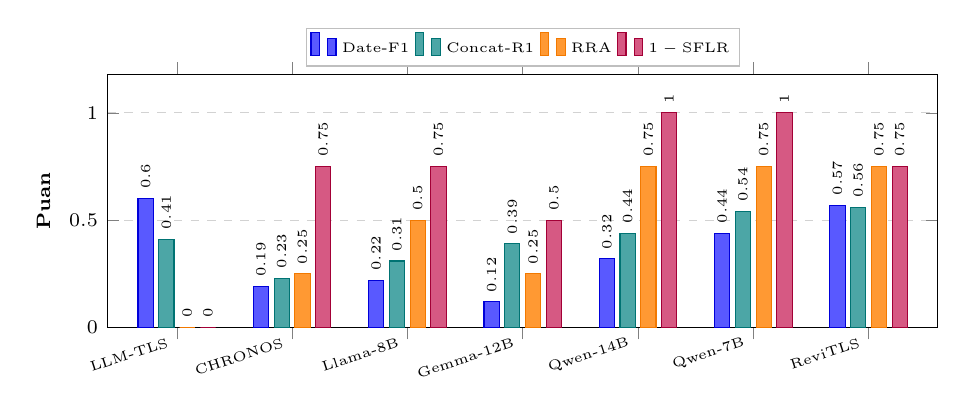
\begin{tikzpicture}
\begin{axis}[
    ybar,
    bar width=5.5pt,
    width=\columnwidth,
    height=4.8cm,
    ymin=0, ymax=1.18,
    ylabel={Puan},
    symbolic x coords={LLM-TLS, CHRONOS, Llama-8B, Gemma-12B, Qwen-14B, Qwen-7B, ReviTLS},
    xtick=data,
    x tick label style={font=\tiny, rotate=18, anchor=east},
    y tick label style={font=\scriptsize},
    ylabel style={font=\scriptsize\bfseries},
    legend style={at={(0.5,1.03)}, anchor=south, legend columns=4, font=\tiny, draw=gray!50, inner sep=1.5pt},
    ymajorgrids=true,
    grid style={dashed, gray!35},
    nodes near coords,
    every node near coord/.append style={font=\tiny, rotate=90, anchor=west, /pgf/number format/fixed, /pgf/number format/precision=2}
]
\addplot[fill=blue!65, draw=blue!85!black] coordinates {
    (LLM-TLS, 0.60) (CHRONOS, 0.19) (Llama-8B, 0.22) (Gemma-12B, 0.12) (Qwen-14B, 0.32) (Qwen-7B, 0.44) (ReviTLS, 0.57)
};
\addplot[fill=teal!70, draw=teal!90!black] coordinates {
    (LLM-TLS, 0.41) (CHRONOS, 0.23) (Llama-8B, 0.31) (Gemma-12B, 0.39) (Qwen-14B, 0.44) (Qwen-7B, 0.54) (ReviTLS, 0.56)
};
\addplot[fill=orange!80, draw=orange!95!black] coordinates {
    (LLM-TLS, 0.00) (CHRONOS, 0.25) (Llama-8B, 0.50) (Gemma-12B, 0.25) (Qwen-14B, 0.75) (Qwen-7B, 0.75) (ReviTLS, 0.75)
};
\addplot[fill=purple!65, draw=purple!85!black] coordinates {
    (LLM-TLS, 0.00) (CHRONOS, 0.75) (Llama-8B, 0.75) (Gemma-12B, 0.50) (Qwen-14B, 1.00) (Qwen-7B, 1.00) (ReviTLS, 0.75)
};
\legend{Date-F1, Concat-R1, RRA, $1-\text{SFLR}$}
\end{axis}
\end{tikzpicture}
\caption{Eski tek-konulu (\texttt{T17/bpoil}, $164$ makale) omurga ve dikkat-mekanizmas{\i} kar\c{s}{\i}la\c{s}t{\i}rmas{\i} (tam-derlem Tablo~\ref{tab:main_results}'ten ayr{\i}).}
\label{fig:backbone_chart}
\end{figure}

\bibliographystyle{IEEEtran}
\bibliography{references}

\end{document}
